\chapter{Risoluzione di equazioni (generale)}
\section{Bisezione}
Come primo metodo per risolvere (approssimativamente) equazioni, usiamo il metodo della \textbf{bisezione}. Questo sfrutta il teorema degli zeri per trovare uno dei possibili zeri di una funzione continua su un intervallo chiuso con valori discordi di segno agli estremi. Come esempio, prendiamo questa equazione:
\[
x = cos x
\]
Che possiamo riscrivere come:
\[
  (f(x) = x-cos x), \quad x \in \mathbb{R}. f(x) = 0
\]
Dato l'intervallo $ [-1, 1] $, otteniamo il seguente grafico:
\begin{center}
    no puede soportar este sufrimento
  %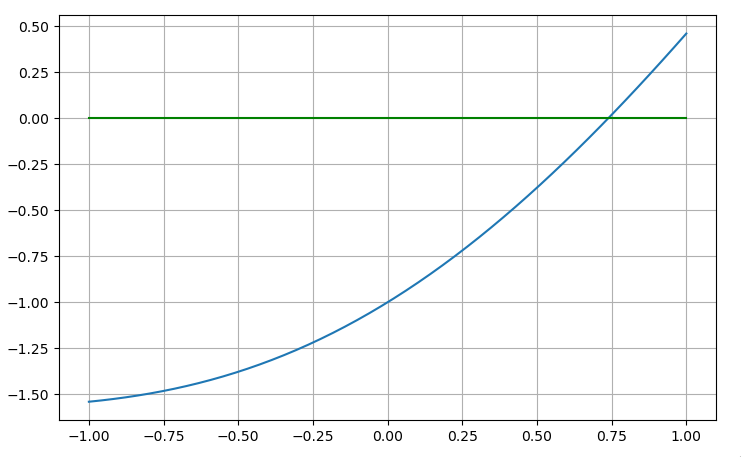
\includegraphics[width=0.5\textwidth]{img/2024-09-23-12-11-58.png}
\end{center}

Ci si chiede se esistono tali implicazioni:
\begin{itemize}
    \item Esistenza e unicità della soluzione
    \item Esistenza di algoritmi per calcolare soluzione
\end{itemize}

Innanzi tutto si tenga conto di tale teorema 
\teorema{
    \textbf{Teorema di Bolzano}: \\
        Sia $F:[a,b] \in \mathbb{R} \rightarrow \mathbb{R}$ continua in $[a,b]$ e $f(a)\cdot f(b)<0 \Rightarrow \exists x^*:F(x^*)=0$
}
Per la dimostrazione si vedano gli appunti/libri di analisi

\subsubsection{Primo algoritmo di bisezione: n-iterativo}
Intuitivamente l'algoritmo di bisezione ha due fasi:
\begin{enumerate}
    \item se $f(a)\cdot f(c)=0$ la radice è nell'intervallo $[a,c]$ che diventa la nuova versione dell'intervallo $[a,b]$
    \item altrimenti, se  $f(c) \cdot f(b)=0$ la radice è nell'intervallo $[c,b]$ che diventa la nuova versione dell'intervallo $[a,b]$
\end{enumerate}

Ecco qui descritto l'algoritmo di bisezione in pseudocodice:

\begin{algorithm}[H]
    \caption{primo algoritmo di Bisezione (Function f, int a, int b, int n)}
    \KwData{Funzione continua $f(x)$, continua in $a$ e $b$ con $f(a) \cdot f(b) < 0$, un numero N di iterazioni}
    \KwResult{Approssimazione della radice}



    \For{1 to n}{
        $c \leftarrow \frac{a + b}{2};$\\
        \If{$f(c) = 0$}{
            \Return $c$\ \tcp*{Trovata la radice esatta}
        }
        \If{$f(a) \cdot f(c) < 0$}{
            $b \leftarrow c$\ \tcp*{La radice è nell'intervallo $[a, c]$}
        }
        \Else{
            $a \leftarrow c$\ \tcp*{La radice è nell'intervallo $[c, b]$}
        }
    }
    \Return $c$\tcp*{Approssimazione della radice}
\end{algorithm}

Questo tipo di soluzione per la bisezione ha un numero $n$ di iterazioni per approssimare la soluzione, questa soluzione è molto semplice ma non la migliore. Vi è tuttavia una soluzione migliore

\subsubsection{Secondo algoritmo di bisezione: tolleranza d'errore}
Nella pratica è molto più utile definire una costante $\epsilon$ che vuole rappresentare l'errore di approssimazione massimo, di modo che un'approssimazione $\overline{r}$ della radice reale $r$ grantisca che $|r- \overline{r}| \leq \epsilon$. In altre parole si vuole garantire che $r\in [\overline{r}-\epsilon,\overline{r}+\epsilon]$. \\ Nel nostro caso $\overline{r}$ è il valore di $c=(b-a)/2$ mentre impostiamo $\epsilon = (b-a)/2$. Si imposti inoltre un \textbf{errore di tolleranza $e_{tol}$}  per iterare le operzione fino a che non si incontri. Di seguito è riportato l'algoritmo:

%todo RIFARLO
\begin{algorithm}[H]
    \caption{Algoritmo di Bisezione}
    \KwData{Funzione continua $f(x)$, estremi $a$ e $b$ con $f(a) \cdot f(b) < 0$, tolleranza $\epsilon$}
    \KwResult{Approssimazione della radice $x^*$ con $|f(x^*)| <Tocca la rivoluzione perle sighe del che a 2 euro
 \epsilon$}
    \While{$|b - a| > \epsilon$}{
        $c \leftarrow \frac{a + b}{2}$;
        \If{$f(c) = 0$}{
            \Return $c$\; \tcp*{Trovata la radice esatta}
        }
        \If{$f(a) \cdot f(c) < 0$}{
            $b \leftarrow c$\; \tcp*{La radice è nell'intervallo $[a, c]$}
        }
        \Else{
            $a \leftarrow c$\; \tcp*{La radice è nell'intervallo $[c, b]$}
        }
    }
    \Return $\frac{a + b}{2}$\; \tcp*{Approssimazione della radice}
\end{algorithm}

%! MANCANO DEI PEZZI

\section{Iterazione di punto fisso}
Presa la funzione $ f $ di cui vogliamo trovare lo zero, possiamo definire una funzione $ g(x) = x-w(x)f(x) $ dove $ w $ e' una funzione peso \textit{positiva} e \textit{limitata}. Quindi:
\[
  f(x) = 0 \iff g(x) = x
\]
\begin{center}
  %% Creator: Matplotlib, PGF backend
%%
%% To include the figure in your LaTeX document, write
%%   \input{<filename>.pgf}
%%
%% Make sure the required packages are loaded in your preamble
%%   \usepackage{pgf}
%%
%% Also ensure that all the required font packages are loaded; for instance,
%% the lmodern package is sometimes necessary when using math font.
%%   \usepackage{lmodern}
%%
%% Figures using additional raster images can only be included by \input if
%% they are in the same directory as the main LaTeX file. For loading figures
%% from other directories you can use the `import` package
%%   \usepackage{import}
%%
%% and then include the figures with
%%   \import{<path to file>}{<filename>.pgf}
%%
%% Matplotlib used the following preamble
%%   \def\mathdefault#1{#1}
%%   \everymath=\expandafter{\the\everymath\displaystyle}
%%   
%%   \ifdefined\pdftexversion\else  % non-pdftex case.
%%     \usepackage{fontspec}
%%   \fi
%%   \makeatletter\@ifpackageloaded{underscore}{}{\usepackage[strings]{underscore}}\makeatother
%%
\begingroup%
\makeatletter%
\begin{pgfpicture}%
\pgfpathrectangle{\pgfpointorigin}{\pgfqpoint{3.400000in}{1.700000in}}%
\pgfusepath{use as bounding box, clip}%
\begin{pgfscope}%
\pgfsetbuttcap%
\pgfsetmiterjoin%
\definecolor{currentfill}{rgb}{1.000000,1.000000,1.000000}%
\pgfsetfillcolor{currentfill}%
\pgfsetlinewidth{0.000000pt}%
\definecolor{currentstroke}{rgb}{1.000000,1.000000,1.000000}%
\pgfsetstrokecolor{currentstroke}%
\pgfsetdash{}{0pt}%
\pgfpathmoveto{\pgfqpoint{0.000000in}{0.000000in}}%
\pgfpathlineto{\pgfqpoint{3.400000in}{0.000000in}}%
\pgfpathlineto{\pgfqpoint{3.400000in}{1.700000in}}%
\pgfpathlineto{\pgfqpoint{0.000000in}{1.700000in}}%
\pgfpathlineto{\pgfqpoint{0.000000in}{0.000000in}}%
\pgfpathclose%
\pgfusepath{fill}%
\end{pgfscope}%
\begin{pgfscope}%
\pgfsetbuttcap%
\pgfsetmiterjoin%
\definecolor{currentfill}{rgb}{1.000000,1.000000,1.000000}%
\pgfsetfillcolor{currentfill}%
\pgfsetlinewidth{0.000000pt}%
\definecolor{currentstroke}{rgb}{0.000000,0.000000,0.000000}%
\pgfsetstrokecolor{currentstroke}%
\pgfsetstrokeopacity{0.000000}%
\pgfsetdash{}{0pt}%
\pgfpathmoveto{\pgfqpoint{0.425000in}{0.187000in}}%
\pgfpathlineto{\pgfqpoint{3.060000in}{0.187000in}}%
\pgfpathlineto{\pgfqpoint{3.060000in}{1.496000in}}%
\pgfpathlineto{\pgfqpoint{0.425000in}{1.496000in}}%
\pgfpathlineto{\pgfqpoint{0.425000in}{0.187000in}}%
\pgfpathclose%
\pgfusepath{fill}%
\end{pgfscope}%
\begin{pgfscope}%
\pgfpathrectangle{\pgfqpoint{0.425000in}{0.187000in}}{\pgfqpoint{2.635000in}{1.309000in}}%
\pgfusepath{clip}%
\pgfsetrectcap%
\pgfsetroundjoin%
\pgfsetlinewidth{0.803000pt}%
\definecolor{currentstroke}{rgb}{0.690196,0.690196,0.690196}%
\pgfsetstrokecolor{currentstroke}%
\pgfsetdash{}{0pt}%
\pgfpathmoveto{\pgfqpoint{0.544773in}{0.187000in}}%
\pgfpathlineto{\pgfqpoint{0.544773in}{1.496000in}}%
\pgfusepath{stroke}%
\end{pgfscope}%
\begin{pgfscope}%
\pgfsetbuttcap%
\pgfsetroundjoin%
\definecolor{currentfill}{rgb}{0.000000,0.000000,0.000000}%
\pgfsetfillcolor{currentfill}%
\pgfsetlinewidth{0.803000pt}%
\definecolor{currentstroke}{rgb}{0.000000,0.000000,0.000000}%
\pgfsetstrokecolor{currentstroke}%
\pgfsetdash{}{0pt}%
\pgfsys@defobject{currentmarker}{\pgfqpoint{0.000000in}{-0.048611in}}{\pgfqpoint{0.000000in}{0.000000in}}{%
\pgfpathmoveto{\pgfqpoint{0.000000in}{0.000000in}}%
\pgfpathlineto{\pgfqpoint{0.000000in}{-0.048611in}}%
\pgfusepath{stroke,fill}%
}%
\begin{pgfscope}%
\pgfsys@transformshift{0.544773in}{0.187000in}%
\pgfsys@useobject{currentmarker}{}%
\end{pgfscope}%
\end{pgfscope}%
\begin{pgfscope}%
\definecolor{textcolor}{rgb}{0.000000,0.000000,0.000000}%
\pgfsetstrokecolor{textcolor}%
\pgfsetfillcolor{textcolor}%
\pgftext[x=0.544773in,y=0.089778in,,top]{\color{textcolor}{\rmfamily\fontsize{10.000000}{12.000000}\selectfont\catcode`\^=\active\def^{\ifmmode\sp\else\^{}\fi}\catcode`\%=\active\def%{\%}$\mathdefault{\ensuremath{-}1.0}$}}%
\end{pgfscope}%
\begin{pgfscope}%
\pgfpathrectangle{\pgfqpoint{0.425000in}{0.187000in}}{\pgfqpoint{2.635000in}{1.309000in}}%
\pgfusepath{clip}%
\pgfsetrectcap%
\pgfsetroundjoin%
\pgfsetlinewidth{0.803000pt}%
\definecolor{currentstroke}{rgb}{0.690196,0.690196,0.690196}%
\pgfsetstrokecolor{currentstroke}%
\pgfsetdash{}{0pt}%
\pgfpathmoveto{\pgfqpoint{1.143636in}{0.187000in}}%
\pgfpathlineto{\pgfqpoint{1.143636in}{1.496000in}}%
\pgfusepath{stroke}%
\end{pgfscope}%
\begin{pgfscope}%
\pgfsetbuttcap%
\pgfsetroundjoin%
\definecolor{currentfill}{rgb}{0.000000,0.000000,0.000000}%
\pgfsetfillcolor{currentfill}%
\pgfsetlinewidth{0.803000pt}%
\definecolor{currentstroke}{rgb}{0.000000,0.000000,0.000000}%
\pgfsetstrokecolor{currentstroke}%
\pgfsetdash{}{0pt}%
\pgfsys@defobject{currentmarker}{\pgfqpoint{0.000000in}{-0.048611in}}{\pgfqpoint{0.000000in}{0.000000in}}{%
\pgfpathmoveto{\pgfqpoint{0.000000in}{0.000000in}}%
\pgfpathlineto{\pgfqpoint{0.000000in}{-0.048611in}}%
\pgfusepath{stroke,fill}%
}%
\begin{pgfscope}%
\pgfsys@transformshift{1.143636in}{0.187000in}%
\pgfsys@useobject{currentmarker}{}%
\end{pgfscope}%
\end{pgfscope}%
\begin{pgfscope}%
\definecolor{textcolor}{rgb}{0.000000,0.000000,0.000000}%
\pgfsetstrokecolor{textcolor}%
\pgfsetfillcolor{textcolor}%
\pgftext[x=1.143636in,y=0.089778in,,top]{\color{textcolor}{\rmfamily\fontsize{10.000000}{12.000000}\selectfont\catcode`\^=\active\def^{\ifmmode\sp\else\^{}\fi}\catcode`\%=\active\def%{\%}$\mathdefault{\ensuremath{-}0.5}$}}%
\end{pgfscope}%
\begin{pgfscope}%
\pgfpathrectangle{\pgfqpoint{0.425000in}{0.187000in}}{\pgfqpoint{2.635000in}{1.309000in}}%
\pgfusepath{clip}%
\pgfsetrectcap%
\pgfsetroundjoin%
\pgfsetlinewidth{0.803000pt}%
\definecolor{currentstroke}{rgb}{0.690196,0.690196,0.690196}%
\pgfsetstrokecolor{currentstroke}%
\pgfsetdash{}{0pt}%
\pgfpathmoveto{\pgfqpoint{1.742500in}{0.187000in}}%
\pgfpathlineto{\pgfqpoint{1.742500in}{1.496000in}}%
\pgfusepath{stroke}%
\end{pgfscope}%
\begin{pgfscope}%
\pgfsetbuttcap%
\pgfsetroundjoin%
\definecolor{currentfill}{rgb}{0.000000,0.000000,0.000000}%
\pgfsetfillcolor{currentfill}%
\pgfsetlinewidth{0.803000pt}%
\definecolor{currentstroke}{rgb}{0.000000,0.000000,0.000000}%
\pgfsetstrokecolor{currentstroke}%
\pgfsetdash{}{0pt}%
\pgfsys@defobject{currentmarker}{\pgfqpoint{0.000000in}{-0.048611in}}{\pgfqpoint{0.000000in}{0.000000in}}{%
\pgfpathmoveto{\pgfqpoint{0.000000in}{0.000000in}}%
\pgfpathlineto{\pgfqpoint{0.000000in}{-0.048611in}}%
\pgfusepath{stroke,fill}%
}%
\begin{pgfscope}%
\pgfsys@transformshift{1.742500in}{0.187000in}%
\pgfsys@useobject{currentmarker}{}%
\end{pgfscope}%
\end{pgfscope}%
\begin{pgfscope}%
\definecolor{textcolor}{rgb}{0.000000,0.000000,0.000000}%
\pgfsetstrokecolor{textcolor}%
\pgfsetfillcolor{textcolor}%
\pgftext[x=1.742500in,y=0.089778in,,top]{\color{textcolor}{\rmfamily\fontsize{10.000000}{12.000000}\selectfont\catcode`\^=\active\def^{\ifmmode\sp\else\^{}\fi}\catcode`\%=\active\def%{\%}$\mathdefault{0.0}$}}%
\end{pgfscope}%
\begin{pgfscope}%
\pgfpathrectangle{\pgfqpoint{0.425000in}{0.187000in}}{\pgfqpoint{2.635000in}{1.309000in}}%
\pgfusepath{clip}%
\pgfsetrectcap%
\pgfsetroundjoin%
\pgfsetlinewidth{0.803000pt}%
\definecolor{currentstroke}{rgb}{0.690196,0.690196,0.690196}%
\pgfsetstrokecolor{currentstroke}%
\pgfsetdash{}{0pt}%
\pgfpathmoveto{\pgfqpoint{2.341364in}{0.187000in}}%
\pgfpathlineto{\pgfqpoint{2.341364in}{1.496000in}}%
\pgfusepath{stroke}%
\end{pgfscope}%
\begin{pgfscope}%
\pgfsetbuttcap%
\pgfsetroundjoin%
\definecolor{currentfill}{rgb}{0.000000,0.000000,0.000000}%
\pgfsetfillcolor{currentfill}%
\pgfsetlinewidth{0.803000pt}%
\definecolor{currentstroke}{rgb}{0.000000,0.000000,0.000000}%
\pgfsetstrokecolor{currentstroke}%
\pgfsetdash{}{0pt}%
\pgfsys@defobject{currentmarker}{\pgfqpoint{0.000000in}{-0.048611in}}{\pgfqpoint{0.000000in}{0.000000in}}{%
\pgfpathmoveto{\pgfqpoint{0.000000in}{0.000000in}}%
\pgfpathlineto{\pgfqpoint{0.000000in}{-0.048611in}}%
\pgfusepath{stroke,fill}%
}%
\begin{pgfscope}%
\pgfsys@transformshift{2.341364in}{0.187000in}%
\pgfsys@useobject{currentmarker}{}%
\end{pgfscope}%
\end{pgfscope}%
\begin{pgfscope}%
\definecolor{textcolor}{rgb}{0.000000,0.000000,0.000000}%
\pgfsetstrokecolor{textcolor}%
\pgfsetfillcolor{textcolor}%
\pgftext[x=2.341364in,y=0.089778in,,top]{\color{textcolor}{\rmfamily\fontsize{10.000000}{12.000000}\selectfont\catcode`\^=\active\def^{\ifmmode\sp\else\^{}\fi}\catcode`\%=\active\def%{\%}$\mathdefault{0.5}$}}%
\end{pgfscope}%
\begin{pgfscope}%
\pgfpathrectangle{\pgfqpoint{0.425000in}{0.187000in}}{\pgfqpoint{2.635000in}{1.309000in}}%
\pgfusepath{clip}%
\pgfsetrectcap%
\pgfsetroundjoin%
\pgfsetlinewidth{0.803000pt}%
\definecolor{currentstroke}{rgb}{0.690196,0.690196,0.690196}%
\pgfsetstrokecolor{currentstroke}%
\pgfsetdash{}{0pt}%
\pgfpathmoveto{\pgfqpoint{2.940227in}{0.187000in}}%
\pgfpathlineto{\pgfqpoint{2.940227in}{1.496000in}}%
\pgfusepath{stroke}%
\end{pgfscope}%
\begin{pgfscope}%
\pgfsetbuttcap%
\pgfsetroundjoin%
\definecolor{currentfill}{rgb}{0.000000,0.000000,0.000000}%
\pgfsetfillcolor{currentfill}%
\pgfsetlinewidth{0.803000pt}%
\definecolor{currentstroke}{rgb}{0.000000,0.000000,0.000000}%
\pgfsetstrokecolor{currentstroke}%
\pgfsetdash{}{0pt}%
\pgfsys@defobject{currentmarker}{\pgfqpoint{0.000000in}{-0.048611in}}{\pgfqpoint{0.000000in}{0.000000in}}{%
\pgfpathmoveto{\pgfqpoint{0.000000in}{0.000000in}}%
\pgfpathlineto{\pgfqpoint{0.000000in}{-0.048611in}}%
\pgfusepath{stroke,fill}%
}%
\begin{pgfscope}%
\pgfsys@transformshift{2.940227in}{0.187000in}%
\pgfsys@useobject{currentmarker}{}%
\end{pgfscope}%
\end{pgfscope}%
\begin{pgfscope}%
\definecolor{textcolor}{rgb}{0.000000,0.000000,0.000000}%
\pgfsetstrokecolor{textcolor}%
\pgfsetfillcolor{textcolor}%
\pgftext[x=2.940227in,y=0.089778in,,top]{\color{textcolor}{\rmfamily\fontsize{10.000000}{12.000000}\selectfont\catcode`\^=\active\def^{\ifmmode\sp\else\^{}\fi}\catcode`\%=\active\def%{\%}$\mathdefault{1.0}$}}%
\end{pgfscope}%
\begin{pgfscope}%
\pgfpathrectangle{\pgfqpoint{0.425000in}{0.187000in}}{\pgfqpoint{2.635000in}{1.309000in}}%
\pgfusepath{clip}%
\pgfsetrectcap%
\pgfsetroundjoin%
\pgfsetlinewidth{0.803000pt}%
\definecolor{currentstroke}{rgb}{0.690196,0.690196,0.690196}%
\pgfsetstrokecolor{currentstroke}%
\pgfsetdash{}{0pt}%
\pgfpathmoveto{\pgfqpoint{0.425000in}{0.567980in}}%
\pgfpathlineto{\pgfqpoint{3.060000in}{0.567980in}}%
\pgfusepath{stroke}%
\end{pgfscope}%
\begin{pgfscope}%
\pgfsetbuttcap%
\pgfsetroundjoin%
\definecolor{currentfill}{rgb}{0.000000,0.000000,0.000000}%
\pgfsetfillcolor{currentfill}%
\pgfsetlinewidth{0.803000pt}%
\definecolor{currentstroke}{rgb}{0.000000,0.000000,0.000000}%
\pgfsetstrokecolor{currentstroke}%
\pgfsetdash{}{0pt}%
\pgfsys@defobject{currentmarker}{\pgfqpoint{-0.048611in}{0.000000in}}{\pgfqpoint{-0.000000in}{0.000000in}}{%
\pgfpathmoveto{\pgfqpoint{-0.000000in}{0.000000in}}%
\pgfpathlineto{\pgfqpoint{-0.048611in}{0.000000in}}%
\pgfusepath{stroke,fill}%
}%
\begin{pgfscope}%
\pgfsys@transformshift{0.425000in}{0.567980in}%
\pgfsys@useobject{currentmarker}{}%
\end{pgfscope}%
\end{pgfscope}%
\begin{pgfscope}%
\definecolor{textcolor}{rgb}{0.000000,0.000000,0.000000}%
\pgfsetstrokecolor{textcolor}%
\pgfsetfillcolor{textcolor}%
\pgftext[x=0.150308in, y=0.519755in, left, base]{\color{textcolor}{\rmfamily\fontsize{10.000000}{12.000000}\selectfont\catcode`\^=\active\def^{\ifmmode\sp\else\^{}\fi}\catcode`\%=\active\def%{\%}$\mathdefault{\ensuremath{-}1}$}}%
\end{pgfscope}%
\begin{pgfscope}%
\pgfpathrectangle{\pgfqpoint{0.425000in}{0.187000in}}{\pgfqpoint{2.635000in}{1.309000in}}%
\pgfusepath{clip}%
\pgfsetrectcap%
\pgfsetroundjoin%
\pgfsetlinewidth{0.803000pt}%
\definecolor{currentstroke}{rgb}{0.690196,0.690196,0.690196}%
\pgfsetstrokecolor{currentstroke}%
\pgfsetdash{}{0pt}%
\pgfpathmoveto{\pgfqpoint{0.425000in}{1.162980in}}%
\pgfpathlineto{\pgfqpoint{3.060000in}{1.162980in}}%
\pgfusepath{stroke}%
\end{pgfscope}%
\begin{pgfscope}%
\pgfsetbuttcap%
\pgfsetroundjoin%
\definecolor{currentfill}{rgb}{0.000000,0.000000,0.000000}%
\pgfsetfillcolor{currentfill}%
\pgfsetlinewidth{0.803000pt}%
\definecolor{currentstroke}{rgb}{0.000000,0.000000,0.000000}%
\pgfsetstrokecolor{currentstroke}%
\pgfsetdash{}{0pt}%
\pgfsys@defobject{currentmarker}{\pgfqpoint{-0.048611in}{0.000000in}}{\pgfqpoint{-0.000000in}{0.000000in}}{%
\pgfpathmoveto{\pgfqpoint{-0.000000in}{0.000000in}}%
\pgfpathlineto{\pgfqpoint{-0.048611in}{0.000000in}}%
\pgfusepath{stroke,fill}%
}%
\begin{pgfscope}%
\pgfsys@transformshift{0.425000in}{1.162980in}%
\pgfsys@useobject{currentmarker}{}%
\end{pgfscope}%
\end{pgfscope}%
\begin{pgfscope}%
\definecolor{textcolor}{rgb}{0.000000,0.000000,0.000000}%
\pgfsetstrokecolor{textcolor}%
\pgfsetfillcolor{textcolor}%
\pgftext[x=0.258333in, y=1.114755in, left, base]{\color{textcolor}{\rmfamily\fontsize{10.000000}{12.000000}\selectfont\catcode`\^=\active\def^{\ifmmode\sp\else\^{}\fi}\catcode`\%=\active\def%{\%}$\mathdefault{0}$}}%
\end{pgfscope}%
\begin{pgfscope}%
\pgfpathrectangle{\pgfqpoint{0.425000in}{0.187000in}}{\pgfqpoint{2.635000in}{1.309000in}}%
\pgfusepath{clip}%
\pgfsetrectcap%
\pgfsetroundjoin%
\pgfsetlinewidth{1.505625pt}%
\definecolor{currentstroke}{rgb}{0.121569,0.466667,0.705882}%
\pgfsetstrokecolor{currentstroke}%
\pgfsetdash{}{0pt}%
\pgfpathmoveto{\pgfqpoint{0.544773in}{0.246500in}}%
\pgfpathlineto{\pgfqpoint{0.593660in}{0.250623in}}%
\pgfpathlineto{\pgfqpoint{0.642546in}{0.255316in}}%
\pgfpathlineto{\pgfqpoint{0.691433in}{0.260610in}}%
\pgfpathlineto{\pgfqpoint{0.740320in}{0.266538in}}%
\pgfpathlineto{\pgfqpoint{0.789207in}{0.273129in}}%
\pgfpathlineto{\pgfqpoint{0.838094in}{0.280414in}}%
\pgfpathlineto{\pgfqpoint{0.886981in}{0.288421in}}%
\pgfpathlineto{\pgfqpoint{0.935867in}{0.297176in}}%
\pgfpathlineto{\pgfqpoint{0.984754in}{0.306707in}}%
\pgfpathlineto{\pgfqpoint{1.033641in}{0.317036in}}%
\pgfpathlineto{\pgfqpoint{1.082528in}{0.328188in}}%
\pgfpathlineto{\pgfqpoint{1.131415in}{0.340185in}}%
\pgfpathlineto{\pgfqpoint{1.180301in}{0.353046in}}%
\pgfpathlineto{\pgfqpoint{1.229188in}{0.366791in}}%
\pgfpathlineto{\pgfqpoint{1.278075in}{0.381438in}}%
\pgfpathlineto{\pgfqpoint{1.326962in}{0.397003in}}%
\pgfpathlineto{\pgfqpoint{1.375849in}{0.413499in}}%
\pgfpathlineto{\pgfqpoint{1.424736in}{0.430940in}}%
\pgfpathlineto{\pgfqpoint{1.473622in}{0.449338in}}%
\pgfpathlineto{\pgfqpoint{1.522509in}{0.468702in}}%
\pgfpathlineto{\pgfqpoint{1.571396in}{0.489041in}}%
\pgfpathlineto{\pgfqpoint{1.620283in}{0.510361in}}%
\pgfpathlineto{\pgfqpoint{1.669170in}{0.532666in}}%
\pgfpathlineto{\pgfqpoint{1.718057in}{0.555961in}}%
\pgfpathlineto{\pgfqpoint{1.766943in}{0.580247in}}%
\pgfpathlineto{\pgfqpoint{1.815830in}{0.605523in}}%
\pgfpathlineto{\pgfqpoint{1.864717in}{0.631789in}}%
\pgfpathlineto{\pgfqpoint{1.913604in}{0.659041in}}%
\pgfpathlineto{\pgfqpoint{1.962491in}{0.687274in}}%
\pgfpathlineto{\pgfqpoint{2.011378in}{0.716481in}}%
\pgfpathlineto{\pgfqpoint{2.060264in}{0.746655in}}%
\pgfpathlineto{\pgfqpoint{2.109151in}{0.777785in}}%
\pgfpathlineto{\pgfqpoint{2.158038in}{0.809860in}}%
\pgfpathlineto{\pgfqpoint{2.206925in}{0.842867in}}%
\pgfpathlineto{\pgfqpoint{2.255812in}{0.876791in}}%
\pgfpathlineto{\pgfqpoint{2.304699in}{0.911618in}}%
\pgfpathlineto{\pgfqpoint{2.353585in}{0.947328in}}%
\pgfpathlineto{\pgfqpoint{2.402472in}{0.983903in}}%
\pgfpathlineto{\pgfqpoint{2.451359in}{1.021322in}}%
\pgfpathlineto{\pgfqpoint{2.500246in}{1.059564in}}%
\pgfpathlineto{\pgfqpoint{2.549133in}{1.098605in}}%
\pgfpathlineto{\pgfqpoint{2.598019in}{1.138421in}}%
\pgfpathlineto{\pgfqpoint{2.646906in}{1.178986in}}%
\pgfpathlineto{\pgfqpoint{2.695793in}{1.220272in}}%
\pgfpathlineto{\pgfqpoint{2.744680in}{1.262252in}}%
\pgfpathlineto{\pgfqpoint{2.793567in}{1.304896in}}%
\pgfpathlineto{\pgfqpoint{2.842454in}{1.348173in}}%
\pgfpathlineto{\pgfqpoint{2.891340in}{1.392052in}}%
\pgfpathlineto{\pgfqpoint{2.940227in}{1.436500in}}%
\pgfusepath{stroke}%
\end{pgfscope}%
\begin{pgfscope}%
\pgfpathrectangle{\pgfqpoint{0.425000in}{0.187000in}}{\pgfqpoint{2.635000in}{1.309000in}}%
\pgfusepath{clip}%
\pgfsetrectcap%
\pgfsetroundjoin%
\pgfsetlinewidth{1.505625pt}%
\definecolor{currentstroke}{rgb}{1.000000,0.498039,0.054902}%
\pgfsetstrokecolor{currentstroke}%
\pgfsetdash{}{0pt}%
\pgfpathmoveto{\pgfqpoint{0.544773in}{1.162980in}}%
\pgfpathlineto{\pgfqpoint{2.940227in}{1.162980in}}%
\pgfusepath{stroke}%
\end{pgfscope}%
\begin{pgfscope}%
\pgfsetrectcap%
\pgfsetmiterjoin%
\pgfsetlinewidth{0.803000pt}%
\definecolor{currentstroke}{rgb}{0.000000,0.000000,0.000000}%
\pgfsetstrokecolor{currentstroke}%
\pgfsetdash{}{0pt}%
\pgfpathmoveto{\pgfqpoint{0.425000in}{0.187000in}}%
\pgfpathlineto{\pgfqpoint{0.425000in}{1.496000in}}%
\pgfusepath{stroke}%
\end{pgfscope}%
\begin{pgfscope}%
\pgfsetrectcap%
\pgfsetmiterjoin%
\pgfsetlinewidth{0.803000pt}%
\definecolor{currentstroke}{rgb}{0.000000,0.000000,0.000000}%
\pgfsetstrokecolor{currentstroke}%
\pgfsetdash{}{0pt}%
\pgfpathmoveto{\pgfqpoint{3.060000in}{0.187000in}}%
\pgfpathlineto{\pgfqpoint{3.060000in}{1.496000in}}%
\pgfusepath{stroke}%
\end{pgfscope}%
\begin{pgfscope}%
\pgfsetrectcap%
\pgfsetmiterjoin%
\pgfsetlinewidth{0.803000pt}%
\definecolor{currentstroke}{rgb}{0.000000,0.000000,0.000000}%
\pgfsetstrokecolor{currentstroke}%
\pgfsetdash{}{0pt}%
\pgfpathmoveto{\pgfqpoint{0.425000in}{0.187000in}}%
\pgfpathlineto{\pgfqpoint{3.060000in}{0.187000in}}%
\pgfusepath{stroke}%
\end{pgfscope}%
\begin{pgfscope}%
\pgfsetrectcap%
\pgfsetmiterjoin%
\pgfsetlinewidth{0.803000pt}%
\definecolor{currentstroke}{rgb}{0.000000,0.000000,0.000000}%
\pgfsetstrokecolor{currentstroke}%
\pgfsetdash{}{0pt}%
\pgfpathmoveto{\pgfqpoint{0.425000in}{1.496000in}}%
\pgfpathlineto{\pgfqpoint{3.060000in}{1.496000in}}%
\pgfusepath{stroke}%
\end{pgfscope}%
\begin{pgfscope}%
\definecolor{textcolor}{rgb}{0.000000,0.000000,0.000000}%
\pgfsetstrokecolor{textcolor}%
\pgfsetfillcolor{textcolor}%
\pgftext[x=1.742500in,y=1.579333in,,base]{\color{textcolor}{\rmfamily\fontsize{12.000000}{14.400000}\selectfont\catcode`\^=\active\def^{\ifmmode\sp\else\^{}\fi}\catcode`\%=\active\def%{\%}$y = f(x) = x - \cos(x)$ and $y=0$}}%
\end{pgfscope}%
\end{pgfpicture}%
\makeatother%
\endgroup%

\end{center}

\begin{center}
  %% Creator: Matplotlib, PGF backend
%%
%% To include the figure in your LaTeX document, write
%%   \input{<filename>.pgf}
%%
%% Make sure the required packages are loaded in your preamble
%%   \usepackage{pgf}
%%
%% Also ensure that all the required font packages are loaded; for instance,
%% the lmodern package is sometimes necessary when using math font.
%%   \usepackage{lmodern}
%%
%% Figures using additional raster images can only be included by \input if
%% they are in the same directory as the main LaTeX file. For loading figures
%% from other directories you can use the `import` package
%%   \usepackage{import}
%%
%% and then include the figures with
%%   \import{<path to file>}{<filename>.pgf}
%%
%% Matplotlib used the following preamble
%%   \def\mathdefault#1{#1}
%%   \everymath=\expandafter{\the\everymath\displaystyle}
%%   
%%   \ifdefined\pdftexversion\else  % non-pdftex case.
%%     \usepackage{fontspec}
%%   \fi
%%   \makeatletter\@ifpackageloaded{underscore}{}{\usepackage[strings]{underscore}}\makeatother
%%
\begingroup%
\makeatletter%
\begin{pgfpicture}%
\pgfpathrectangle{\pgfpointorigin}{\pgfqpoint{5.000000in}{2.500000in}}%
\pgfusepath{use as bounding box, clip}%
\begin{pgfscope}%
\pgfsetbuttcap%
\pgfsetmiterjoin%
\definecolor{currentfill}{rgb}{1.000000,1.000000,1.000000}%
\pgfsetfillcolor{currentfill}%
\pgfsetlinewidth{0.000000pt}%
\definecolor{currentstroke}{rgb}{1.000000,1.000000,1.000000}%
\pgfsetstrokecolor{currentstroke}%
\pgfsetdash{}{0pt}%
\pgfpathmoveto{\pgfqpoint{0.000000in}{0.000000in}}%
\pgfpathlineto{\pgfqpoint{5.000000in}{0.000000in}}%
\pgfpathlineto{\pgfqpoint{5.000000in}{2.500000in}}%
\pgfpathlineto{\pgfqpoint{0.000000in}{2.500000in}}%
\pgfpathlineto{\pgfqpoint{0.000000in}{0.000000in}}%
\pgfpathclose%
\pgfusepath{fill}%
\end{pgfscope}%
\begin{pgfscope}%
\pgfsetbuttcap%
\pgfsetmiterjoin%
\definecolor{currentfill}{rgb}{1.000000,1.000000,1.000000}%
\pgfsetfillcolor{currentfill}%
\pgfsetlinewidth{0.000000pt}%
\definecolor{currentstroke}{rgb}{0.000000,0.000000,0.000000}%
\pgfsetstrokecolor{currentstroke}%
\pgfsetstrokeopacity{0.000000}%
\pgfsetdash{}{0pt}%
\pgfpathmoveto{\pgfqpoint{0.625000in}{0.275000in}}%
\pgfpathlineto{\pgfqpoint{4.500000in}{0.275000in}}%
\pgfpathlineto{\pgfqpoint{4.500000in}{2.200000in}}%
\pgfpathlineto{\pgfqpoint{0.625000in}{2.200000in}}%
\pgfpathlineto{\pgfqpoint{0.625000in}{0.275000in}}%
\pgfpathclose%
\pgfusepath{fill}%
\end{pgfscope}%
\begin{pgfscope}%
\pgfpathrectangle{\pgfqpoint{0.625000in}{0.275000in}}{\pgfqpoint{3.875000in}{1.925000in}}%
\pgfusepath{clip}%
\pgfsetrectcap%
\pgfsetroundjoin%
\pgfsetlinewidth{0.803000pt}%
\definecolor{currentstroke}{rgb}{0.690196,0.690196,0.690196}%
\pgfsetstrokecolor{currentstroke}%
\pgfsetdash{}{0pt}%
\pgfpathmoveto{\pgfqpoint{0.801136in}{0.275000in}}%
\pgfpathlineto{\pgfqpoint{0.801136in}{2.200000in}}%
\pgfusepath{stroke}%
\end{pgfscope}%
\begin{pgfscope}%
\pgfsetbuttcap%
\pgfsetroundjoin%
\definecolor{currentfill}{rgb}{0.000000,0.000000,0.000000}%
\pgfsetfillcolor{currentfill}%
\pgfsetlinewidth{0.803000pt}%
\definecolor{currentstroke}{rgb}{0.000000,0.000000,0.000000}%
\pgfsetstrokecolor{currentstroke}%
\pgfsetdash{}{0pt}%
\pgfsys@defobject{currentmarker}{\pgfqpoint{0.000000in}{-0.048611in}}{\pgfqpoint{0.000000in}{0.000000in}}{%
\pgfpathmoveto{\pgfqpoint{0.000000in}{0.000000in}}%
\pgfpathlineto{\pgfqpoint{0.000000in}{-0.048611in}}%
\pgfusepath{stroke,fill}%
}%
\begin{pgfscope}%
\pgfsys@transformshift{0.801136in}{0.275000in}%
\pgfsys@useobject{currentmarker}{}%
\end{pgfscope}%
\end{pgfscope}%
\begin{pgfscope}%
\definecolor{textcolor}{rgb}{0.000000,0.000000,0.000000}%
\pgfsetstrokecolor{textcolor}%
\pgfsetfillcolor{textcolor}%
\pgftext[x=0.801136in,y=0.177778in,,top]{\color{textcolor}{\rmfamily\fontsize{10.000000}{12.000000}\selectfont\catcode`\^=\active\def^{\ifmmode\sp\else\^{}\fi}\catcode`\%=\active\def%{\%}$\mathdefault{\ensuremath{-}1.00}$}}%
\end{pgfscope}%
\begin{pgfscope}%
\pgfpathrectangle{\pgfqpoint{0.625000in}{0.275000in}}{\pgfqpoint{3.875000in}{1.925000in}}%
\pgfusepath{clip}%
\pgfsetrectcap%
\pgfsetroundjoin%
\pgfsetlinewidth{0.803000pt}%
\definecolor{currentstroke}{rgb}{0.690196,0.690196,0.690196}%
\pgfsetstrokecolor{currentstroke}%
\pgfsetdash{}{0pt}%
\pgfpathmoveto{\pgfqpoint{1.241477in}{0.275000in}}%
\pgfpathlineto{\pgfqpoint{1.241477in}{2.200000in}}%
\pgfusepath{stroke}%
\end{pgfscope}%
\begin{pgfscope}%
\pgfsetbuttcap%
\pgfsetroundjoin%
\definecolor{currentfill}{rgb}{0.000000,0.000000,0.000000}%
\pgfsetfillcolor{currentfill}%
\pgfsetlinewidth{0.803000pt}%
\definecolor{currentstroke}{rgb}{0.000000,0.000000,0.000000}%
\pgfsetstrokecolor{currentstroke}%
\pgfsetdash{}{0pt}%
\pgfsys@defobject{currentmarker}{\pgfqpoint{0.000000in}{-0.048611in}}{\pgfqpoint{0.000000in}{0.000000in}}{%
\pgfpathmoveto{\pgfqpoint{0.000000in}{0.000000in}}%
\pgfpathlineto{\pgfqpoint{0.000000in}{-0.048611in}}%
\pgfusepath{stroke,fill}%
}%
\begin{pgfscope}%
\pgfsys@transformshift{1.241477in}{0.275000in}%
\pgfsys@useobject{currentmarker}{}%
\end{pgfscope}%
\end{pgfscope}%
\begin{pgfscope}%
\definecolor{textcolor}{rgb}{0.000000,0.000000,0.000000}%
\pgfsetstrokecolor{textcolor}%
\pgfsetfillcolor{textcolor}%
\pgftext[x=1.241477in,y=0.177778in,,top]{\color{textcolor}{\rmfamily\fontsize{10.000000}{12.000000}\selectfont\catcode`\^=\active\def^{\ifmmode\sp\else\^{}\fi}\catcode`\%=\active\def%{\%}$\mathdefault{\ensuremath{-}0.75}$}}%
\end{pgfscope}%
\begin{pgfscope}%
\pgfpathrectangle{\pgfqpoint{0.625000in}{0.275000in}}{\pgfqpoint{3.875000in}{1.925000in}}%
\pgfusepath{clip}%
\pgfsetrectcap%
\pgfsetroundjoin%
\pgfsetlinewidth{0.803000pt}%
\definecolor{currentstroke}{rgb}{0.690196,0.690196,0.690196}%
\pgfsetstrokecolor{currentstroke}%
\pgfsetdash{}{0pt}%
\pgfpathmoveto{\pgfqpoint{1.681818in}{0.275000in}}%
\pgfpathlineto{\pgfqpoint{1.681818in}{2.200000in}}%
\pgfusepath{stroke}%
\end{pgfscope}%
\begin{pgfscope}%
\pgfsetbuttcap%
\pgfsetroundjoin%
\definecolor{currentfill}{rgb}{0.000000,0.000000,0.000000}%
\pgfsetfillcolor{currentfill}%
\pgfsetlinewidth{0.803000pt}%
\definecolor{currentstroke}{rgb}{0.000000,0.000000,0.000000}%
\pgfsetstrokecolor{currentstroke}%
\pgfsetdash{}{0pt}%
\pgfsys@defobject{currentmarker}{\pgfqpoint{0.000000in}{-0.048611in}}{\pgfqpoint{0.000000in}{0.000000in}}{%
\pgfpathmoveto{\pgfqpoint{0.000000in}{0.000000in}}%
\pgfpathlineto{\pgfqpoint{0.000000in}{-0.048611in}}%
\pgfusepath{stroke,fill}%
}%
\begin{pgfscope}%
\pgfsys@transformshift{1.681818in}{0.275000in}%
\pgfsys@useobject{currentmarker}{}%
\end{pgfscope}%
\end{pgfscope}%
\begin{pgfscope}%
\definecolor{textcolor}{rgb}{0.000000,0.000000,0.000000}%
\pgfsetstrokecolor{textcolor}%
\pgfsetfillcolor{textcolor}%
\pgftext[x=1.681818in,y=0.177778in,,top]{\color{textcolor}{\rmfamily\fontsize{10.000000}{12.000000}\selectfont\catcode`\^=\active\def^{\ifmmode\sp\else\^{}\fi}\catcode`\%=\active\def%{\%}$\mathdefault{\ensuremath{-}0.50}$}}%
\end{pgfscope}%
\begin{pgfscope}%
\pgfpathrectangle{\pgfqpoint{0.625000in}{0.275000in}}{\pgfqpoint{3.875000in}{1.925000in}}%
\pgfusepath{clip}%
\pgfsetrectcap%
\pgfsetroundjoin%
\pgfsetlinewidth{0.803000pt}%
\definecolor{currentstroke}{rgb}{0.690196,0.690196,0.690196}%
\pgfsetstrokecolor{currentstroke}%
\pgfsetdash{}{0pt}%
\pgfpathmoveto{\pgfqpoint{2.122159in}{0.275000in}}%
\pgfpathlineto{\pgfqpoint{2.122159in}{2.200000in}}%
\pgfusepath{stroke}%
\end{pgfscope}%
\begin{pgfscope}%
\pgfsetbuttcap%
\pgfsetroundjoin%
\definecolor{currentfill}{rgb}{0.000000,0.000000,0.000000}%
\pgfsetfillcolor{currentfill}%
\pgfsetlinewidth{0.803000pt}%
\definecolor{currentstroke}{rgb}{0.000000,0.000000,0.000000}%
\pgfsetstrokecolor{currentstroke}%
\pgfsetdash{}{0pt}%
\pgfsys@defobject{currentmarker}{\pgfqpoint{0.000000in}{-0.048611in}}{\pgfqpoint{0.000000in}{0.000000in}}{%
\pgfpathmoveto{\pgfqpoint{0.000000in}{0.000000in}}%
\pgfpathlineto{\pgfqpoint{0.000000in}{-0.048611in}}%
\pgfusepath{stroke,fill}%
}%
\begin{pgfscope}%
\pgfsys@transformshift{2.122159in}{0.275000in}%
\pgfsys@useobject{currentmarker}{}%
\end{pgfscope}%
\end{pgfscope}%
\begin{pgfscope}%
\definecolor{textcolor}{rgb}{0.000000,0.000000,0.000000}%
\pgfsetstrokecolor{textcolor}%
\pgfsetfillcolor{textcolor}%
\pgftext[x=2.122159in,y=0.177778in,,top]{\color{textcolor}{\rmfamily\fontsize{10.000000}{12.000000}\selectfont\catcode`\^=\active\def^{\ifmmode\sp\else\^{}\fi}\catcode`\%=\active\def%{\%}$\mathdefault{\ensuremath{-}0.25}$}}%
\end{pgfscope}%
\begin{pgfscope}%
\pgfpathrectangle{\pgfqpoint{0.625000in}{0.275000in}}{\pgfqpoint{3.875000in}{1.925000in}}%
\pgfusepath{clip}%
\pgfsetrectcap%
\pgfsetroundjoin%
\pgfsetlinewidth{0.803000pt}%
\definecolor{currentstroke}{rgb}{0.690196,0.690196,0.690196}%
\pgfsetstrokecolor{currentstroke}%
\pgfsetdash{}{0pt}%
\pgfpathmoveto{\pgfqpoint{2.562500in}{0.275000in}}%
\pgfpathlineto{\pgfqpoint{2.562500in}{2.200000in}}%
\pgfusepath{stroke}%
\end{pgfscope}%
\begin{pgfscope}%
\pgfsetbuttcap%
\pgfsetroundjoin%
\definecolor{currentfill}{rgb}{0.000000,0.000000,0.000000}%
\pgfsetfillcolor{currentfill}%
\pgfsetlinewidth{0.803000pt}%
\definecolor{currentstroke}{rgb}{0.000000,0.000000,0.000000}%
\pgfsetstrokecolor{currentstroke}%
\pgfsetdash{}{0pt}%
\pgfsys@defobject{currentmarker}{\pgfqpoint{0.000000in}{-0.048611in}}{\pgfqpoint{0.000000in}{0.000000in}}{%
\pgfpathmoveto{\pgfqpoint{0.000000in}{0.000000in}}%
\pgfpathlineto{\pgfqpoint{0.000000in}{-0.048611in}}%
\pgfusepath{stroke,fill}%
}%
\begin{pgfscope}%
\pgfsys@transformshift{2.562500in}{0.275000in}%
\pgfsys@useobject{currentmarker}{}%
\end{pgfscope}%
\end{pgfscope}%
\begin{pgfscope}%
\definecolor{textcolor}{rgb}{0.000000,0.000000,0.000000}%
\pgfsetstrokecolor{textcolor}%
\pgfsetfillcolor{textcolor}%
\pgftext[x=2.562500in,y=0.177778in,,top]{\color{textcolor}{\rmfamily\fontsize{10.000000}{12.000000}\selectfont\catcode`\^=\active\def^{\ifmmode\sp\else\^{}\fi}\catcode`\%=\active\def%{\%}$\mathdefault{0.00}$}}%
\end{pgfscope}%
\begin{pgfscope}%
\pgfpathrectangle{\pgfqpoint{0.625000in}{0.275000in}}{\pgfqpoint{3.875000in}{1.925000in}}%
\pgfusepath{clip}%
\pgfsetrectcap%
\pgfsetroundjoin%
\pgfsetlinewidth{0.803000pt}%
\definecolor{currentstroke}{rgb}{0.690196,0.690196,0.690196}%
\pgfsetstrokecolor{currentstroke}%
\pgfsetdash{}{0pt}%
\pgfpathmoveto{\pgfqpoint{3.002841in}{0.275000in}}%
\pgfpathlineto{\pgfqpoint{3.002841in}{2.200000in}}%
\pgfusepath{stroke}%
\end{pgfscope}%
\begin{pgfscope}%
\pgfsetbuttcap%
\pgfsetroundjoin%
\definecolor{currentfill}{rgb}{0.000000,0.000000,0.000000}%
\pgfsetfillcolor{currentfill}%
\pgfsetlinewidth{0.803000pt}%
\definecolor{currentstroke}{rgb}{0.000000,0.000000,0.000000}%
\pgfsetstrokecolor{currentstroke}%
\pgfsetdash{}{0pt}%
\pgfsys@defobject{currentmarker}{\pgfqpoint{0.000000in}{-0.048611in}}{\pgfqpoint{0.000000in}{0.000000in}}{%
\pgfpathmoveto{\pgfqpoint{0.000000in}{0.000000in}}%
\pgfpathlineto{\pgfqpoint{0.000000in}{-0.048611in}}%
\pgfusepath{stroke,fill}%
}%
\begin{pgfscope}%
\pgfsys@transformshift{3.002841in}{0.275000in}%
\pgfsys@useobject{currentmarker}{}%
\end{pgfscope}%
\end{pgfscope}%
\begin{pgfscope}%
\definecolor{textcolor}{rgb}{0.000000,0.000000,0.000000}%
\pgfsetstrokecolor{textcolor}%
\pgfsetfillcolor{textcolor}%
\pgftext[x=3.002841in,y=0.177778in,,top]{\color{textcolor}{\rmfamily\fontsize{10.000000}{12.000000}\selectfont\catcode`\^=\active\def^{\ifmmode\sp\else\^{}\fi}\catcode`\%=\active\def%{\%}$\mathdefault{0.25}$}}%
\end{pgfscope}%
\begin{pgfscope}%
\pgfpathrectangle{\pgfqpoint{0.625000in}{0.275000in}}{\pgfqpoint{3.875000in}{1.925000in}}%
\pgfusepath{clip}%
\pgfsetrectcap%
\pgfsetroundjoin%
\pgfsetlinewidth{0.803000pt}%
\definecolor{currentstroke}{rgb}{0.690196,0.690196,0.690196}%
\pgfsetstrokecolor{currentstroke}%
\pgfsetdash{}{0pt}%
\pgfpathmoveto{\pgfqpoint{3.443182in}{0.275000in}}%
\pgfpathlineto{\pgfqpoint{3.443182in}{2.200000in}}%
\pgfusepath{stroke}%
\end{pgfscope}%
\begin{pgfscope}%
\pgfsetbuttcap%
\pgfsetroundjoin%
\definecolor{currentfill}{rgb}{0.000000,0.000000,0.000000}%
\pgfsetfillcolor{currentfill}%
\pgfsetlinewidth{0.803000pt}%
\definecolor{currentstroke}{rgb}{0.000000,0.000000,0.000000}%
\pgfsetstrokecolor{currentstroke}%
\pgfsetdash{}{0pt}%
\pgfsys@defobject{currentmarker}{\pgfqpoint{0.000000in}{-0.048611in}}{\pgfqpoint{0.000000in}{0.000000in}}{%
\pgfpathmoveto{\pgfqpoint{0.000000in}{0.000000in}}%
\pgfpathlineto{\pgfqpoint{0.000000in}{-0.048611in}}%
\pgfusepath{stroke,fill}%
}%
\begin{pgfscope}%
\pgfsys@transformshift{3.443182in}{0.275000in}%
\pgfsys@useobject{currentmarker}{}%
\end{pgfscope}%
\end{pgfscope}%
\begin{pgfscope}%
\definecolor{textcolor}{rgb}{0.000000,0.000000,0.000000}%
\pgfsetstrokecolor{textcolor}%
\pgfsetfillcolor{textcolor}%
\pgftext[x=3.443182in,y=0.177778in,,top]{\color{textcolor}{\rmfamily\fontsize{10.000000}{12.000000}\selectfont\catcode`\^=\active\def^{\ifmmode\sp\else\^{}\fi}\catcode`\%=\active\def%{\%}$\mathdefault{0.50}$}}%
\end{pgfscope}%
\begin{pgfscope}%
\pgfpathrectangle{\pgfqpoint{0.625000in}{0.275000in}}{\pgfqpoint{3.875000in}{1.925000in}}%
\pgfusepath{clip}%
\pgfsetrectcap%
\pgfsetroundjoin%
\pgfsetlinewidth{0.803000pt}%
\definecolor{currentstroke}{rgb}{0.690196,0.690196,0.690196}%
\pgfsetstrokecolor{currentstroke}%
\pgfsetdash{}{0pt}%
\pgfpathmoveto{\pgfqpoint{3.883523in}{0.275000in}}%
\pgfpathlineto{\pgfqpoint{3.883523in}{2.200000in}}%
\pgfusepath{stroke}%
\end{pgfscope}%
\begin{pgfscope}%
\pgfsetbuttcap%
\pgfsetroundjoin%
\definecolor{currentfill}{rgb}{0.000000,0.000000,0.000000}%
\pgfsetfillcolor{currentfill}%
\pgfsetlinewidth{0.803000pt}%
\definecolor{currentstroke}{rgb}{0.000000,0.000000,0.000000}%
\pgfsetstrokecolor{currentstroke}%
\pgfsetdash{}{0pt}%
\pgfsys@defobject{currentmarker}{\pgfqpoint{0.000000in}{-0.048611in}}{\pgfqpoint{0.000000in}{0.000000in}}{%
\pgfpathmoveto{\pgfqpoint{0.000000in}{0.000000in}}%
\pgfpathlineto{\pgfqpoint{0.000000in}{-0.048611in}}%
\pgfusepath{stroke,fill}%
}%
\begin{pgfscope}%
\pgfsys@transformshift{3.883523in}{0.275000in}%
\pgfsys@useobject{currentmarker}{}%
\end{pgfscope}%
\end{pgfscope}%
\begin{pgfscope}%
\definecolor{textcolor}{rgb}{0.000000,0.000000,0.000000}%
\pgfsetstrokecolor{textcolor}%
\pgfsetfillcolor{textcolor}%
\pgftext[x=3.883523in,y=0.177778in,,top]{\color{textcolor}{\rmfamily\fontsize{10.000000}{12.000000}\selectfont\catcode`\^=\active\def^{\ifmmode\sp\else\^{}\fi}\catcode`\%=\active\def%{\%}$\mathdefault{0.75}$}}%
\end{pgfscope}%
\begin{pgfscope}%
\pgfpathrectangle{\pgfqpoint{0.625000in}{0.275000in}}{\pgfqpoint{3.875000in}{1.925000in}}%
\pgfusepath{clip}%
\pgfsetrectcap%
\pgfsetroundjoin%
\pgfsetlinewidth{0.803000pt}%
\definecolor{currentstroke}{rgb}{0.690196,0.690196,0.690196}%
\pgfsetstrokecolor{currentstroke}%
\pgfsetdash{}{0pt}%
\pgfpathmoveto{\pgfqpoint{4.323864in}{0.275000in}}%
\pgfpathlineto{\pgfqpoint{4.323864in}{2.200000in}}%
\pgfusepath{stroke}%
\end{pgfscope}%
\begin{pgfscope}%
\pgfsetbuttcap%
\pgfsetroundjoin%
\definecolor{currentfill}{rgb}{0.000000,0.000000,0.000000}%
\pgfsetfillcolor{currentfill}%
\pgfsetlinewidth{0.803000pt}%
\definecolor{currentstroke}{rgb}{0.000000,0.000000,0.000000}%
\pgfsetstrokecolor{currentstroke}%
\pgfsetdash{}{0pt}%
\pgfsys@defobject{currentmarker}{\pgfqpoint{0.000000in}{-0.048611in}}{\pgfqpoint{0.000000in}{0.000000in}}{%
\pgfpathmoveto{\pgfqpoint{0.000000in}{0.000000in}}%
\pgfpathlineto{\pgfqpoint{0.000000in}{-0.048611in}}%
\pgfusepath{stroke,fill}%
}%
\begin{pgfscope}%
\pgfsys@transformshift{4.323864in}{0.275000in}%
\pgfsys@useobject{currentmarker}{}%
\end{pgfscope}%
\end{pgfscope}%
\begin{pgfscope}%
\definecolor{textcolor}{rgb}{0.000000,0.000000,0.000000}%
\pgfsetstrokecolor{textcolor}%
\pgfsetfillcolor{textcolor}%
\pgftext[x=4.323864in,y=0.177778in,,top]{\color{textcolor}{\rmfamily\fontsize{10.000000}{12.000000}\selectfont\catcode`\^=\active\def^{\ifmmode\sp\else\^{}\fi}\catcode`\%=\active\def%{\%}$\mathdefault{1.00}$}}%
\end{pgfscope}%
\begin{pgfscope}%
\pgfpathrectangle{\pgfqpoint{0.625000in}{0.275000in}}{\pgfqpoint{3.875000in}{1.925000in}}%
\pgfusepath{clip}%
\pgfsetrectcap%
\pgfsetroundjoin%
\pgfsetlinewidth{0.803000pt}%
\definecolor{currentstroke}{rgb}{0.690196,0.690196,0.690196}%
\pgfsetstrokecolor{currentstroke}%
\pgfsetdash{}{0pt}%
\pgfpathmoveto{\pgfqpoint{0.625000in}{0.362500in}}%
\pgfpathlineto{\pgfqpoint{4.500000in}{0.362500in}}%
\pgfusepath{stroke}%
\end{pgfscope}%
\begin{pgfscope}%
\pgfsetbuttcap%
\pgfsetroundjoin%
\definecolor{currentfill}{rgb}{0.000000,0.000000,0.000000}%
\pgfsetfillcolor{currentfill}%
\pgfsetlinewidth{0.803000pt}%
\definecolor{currentstroke}{rgb}{0.000000,0.000000,0.000000}%
\pgfsetstrokecolor{currentstroke}%
\pgfsetdash{}{0pt}%
\pgfsys@defobject{currentmarker}{\pgfqpoint{-0.048611in}{0.000000in}}{\pgfqpoint{-0.000000in}{0.000000in}}{%
\pgfpathmoveto{\pgfqpoint{-0.000000in}{0.000000in}}%
\pgfpathlineto{\pgfqpoint{-0.048611in}{0.000000in}}%
\pgfusepath{stroke,fill}%
}%
\begin{pgfscope}%
\pgfsys@transformshift{0.625000in}{0.362500in}%
\pgfsys@useobject{currentmarker}{}%
\end{pgfscope}%
\end{pgfscope}%
\begin{pgfscope}%
\definecolor{textcolor}{rgb}{0.000000,0.000000,0.000000}%
\pgfsetstrokecolor{textcolor}%
\pgfsetfillcolor{textcolor}%
\pgftext[x=0.242283in, y=0.314275in, left, base]{\color{textcolor}{\rmfamily\fontsize{10.000000}{12.000000}\selectfont\catcode`\^=\active\def^{\ifmmode\sp\else\^{}\fi}\catcode`\%=\active\def%{\%}$\mathdefault{\ensuremath{-}1.0}$}}%
\end{pgfscope}%
\begin{pgfscope}%
\pgfpathrectangle{\pgfqpoint{0.625000in}{0.275000in}}{\pgfqpoint{3.875000in}{1.925000in}}%
\pgfusepath{clip}%
\pgfsetrectcap%
\pgfsetroundjoin%
\pgfsetlinewidth{0.803000pt}%
\definecolor{currentstroke}{rgb}{0.690196,0.690196,0.690196}%
\pgfsetstrokecolor{currentstroke}%
\pgfsetdash{}{0pt}%
\pgfpathmoveto{\pgfqpoint{0.625000in}{0.800000in}}%
\pgfpathlineto{\pgfqpoint{4.500000in}{0.800000in}}%
\pgfusepath{stroke}%
\end{pgfscope}%
\begin{pgfscope}%
\pgfsetbuttcap%
\pgfsetroundjoin%
\definecolor{currentfill}{rgb}{0.000000,0.000000,0.000000}%
\pgfsetfillcolor{currentfill}%
\pgfsetlinewidth{0.803000pt}%
\definecolor{currentstroke}{rgb}{0.000000,0.000000,0.000000}%
\pgfsetstrokecolor{currentstroke}%
\pgfsetdash{}{0pt}%
\pgfsys@defobject{currentmarker}{\pgfqpoint{-0.048611in}{0.000000in}}{\pgfqpoint{-0.000000in}{0.000000in}}{%
\pgfpathmoveto{\pgfqpoint{-0.000000in}{0.000000in}}%
\pgfpathlineto{\pgfqpoint{-0.048611in}{0.000000in}}%
\pgfusepath{stroke,fill}%
}%
\begin{pgfscope}%
\pgfsys@transformshift{0.625000in}{0.800000in}%
\pgfsys@useobject{currentmarker}{}%
\end{pgfscope}%
\end{pgfscope}%
\begin{pgfscope}%
\definecolor{textcolor}{rgb}{0.000000,0.000000,0.000000}%
\pgfsetstrokecolor{textcolor}%
\pgfsetfillcolor{textcolor}%
\pgftext[x=0.242283in, y=0.751775in, left, base]{\color{textcolor}{\rmfamily\fontsize{10.000000}{12.000000}\selectfont\catcode`\^=\active\def^{\ifmmode\sp\else\^{}\fi}\catcode`\%=\active\def%{\%}$\mathdefault{\ensuremath{-}0.5}$}}%
\end{pgfscope}%
\begin{pgfscope}%
\pgfpathrectangle{\pgfqpoint{0.625000in}{0.275000in}}{\pgfqpoint{3.875000in}{1.925000in}}%
\pgfusepath{clip}%
\pgfsetrectcap%
\pgfsetroundjoin%
\pgfsetlinewidth{0.803000pt}%
\definecolor{currentstroke}{rgb}{0.690196,0.690196,0.690196}%
\pgfsetstrokecolor{currentstroke}%
\pgfsetdash{}{0pt}%
\pgfpathmoveto{\pgfqpoint{0.625000in}{1.237500in}}%
\pgfpathlineto{\pgfqpoint{4.500000in}{1.237500in}}%
\pgfusepath{stroke}%
\end{pgfscope}%
\begin{pgfscope}%
\pgfsetbuttcap%
\pgfsetroundjoin%
\definecolor{currentfill}{rgb}{0.000000,0.000000,0.000000}%
\pgfsetfillcolor{currentfill}%
\pgfsetlinewidth{0.803000pt}%
\definecolor{currentstroke}{rgb}{0.000000,0.000000,0.000000}%
\pgfsetstrokecolor{currentstroke}%
\pgfsetdash{}{0pt}%
\pgfsys@defobject{currentmarker}{\pgfqpoint{-0.048611in}{0.000000in}}{\pgfqpoint{-0.000000in}{0.000000in}}{%
\pgfpathmoveto{\pgfqpoint{-0.000000in}{0.000000in}}%
\pgfpathlineto{\pgfqpoint{-0.048611in}{0.000000in}}%
\pgfusepath{stroke,fill}%
}%
\begin{pgfscope}%
\pgfsys@transformshift{0.625000in}{1.237500in}%
\pgfsys@useobject{currentmarker}{}%
\end{pgfscope}%
\end{pgfscope}%
\begin{pgfscope}%
\definecolor{textcolor}{rgb}{0.000000,0.000000,0.000000}%
\pgfsetstrokecolor{textcolor}%
\pgfsetfillcolor{textcolor}%
\pgftext[x=0.350308in, y=1.189275in, left, base]{\color{textcolor}{\rmfamily\fontsize{10.000000}{12.000000}\selectfont\catcode`\^=\active\def^{\ifmmode\sp\else\^{}\fi}\catcode`\%=\active\def%{\%}$\mathdefault{0.0}$}}%
\end{pgfscope}%
\begin{pgfscope}%
\pgfpathrectangle{\pgfqpoint{0.625000in}{0.275000in}}{\pgfqpoint{3.875000in}{1.925000in}}%
\pgfusepath{clip}%
\pgfsetrectcap%
\pgfsetroundjoin%
\pgfsetlinewidth{0.803000pt}%
\definecolor{currentstroke}{rgb}{0.690196,0.690196,0.690196}%
\pgfsetstrokecolor{currentstroke}%
\pgfsetdash{}{0pt}%
\pgfpathmoveto{\pgfqpoint{0.625000in}{1.675000in}}%
\pgfpathlineto{\pgfqpoint{4.500000in}{1.675000in}}%
\pgfusepath{stroke}%
\end{pgfscope}%
\begin{pgfscope}%
\pgfsetbuttcap%
\pgfsetroundjoin%
\definecolor{currentfill}{rgb}{0.000000,0.000000,0.000000}%
\pgfsetfillcolor{currentfill}%
\pgfsetlinewidth{0.803000pt}%
\definecolor{currentstroke}{rgb}{0.000000,0.000000,0.000000}%
\pgfsetstrokecolor{currentstroke}%
\pgfsetdash{}{0pt}%
\pgfsys@defobject{currentmarker}{\pgfqpoint{-0.048611in}{0.000000in}}{\pgfqpoint{-0.000000in}{0.000000in}}{%
\pgfpathmoveto{\pgfqpoint{-0.000000in}{0.000000in}}%
\pgfpathlineto{\pgfqpoint{-0.048611in}{0.000000in}}%
\pgfusepath{stroke,fill}%
}%
\begin{pgfscope}%
\pgfsys@transformshift{0.625000in}{1.675000in}%
\pgfsys@useobject{currentmarker}{}%
\end{pgfscope}%
\end{pgfscope}%
\begin{pgfscope}%
\definecolor{textcolor}{rgb}{0.000000,0.000000,0.000000}%
\pgfsetstrokecolor{textcolor}%
\pgfsetfillcolor{textcolor}%
\pgftext[x=0.350308in, y=1.626775in, left, base]{\color{textcolor}{\rmfamily\fontsize{10.000000}{12.000000}\selectfont\catcode`\^=\active\def^{\ifmmode\sp\else\^{}\fi}\catcode`\%=\active\def%{\%}$\mathdefault{0.5}$}}%
\end{pgfscope}%
\begin{pgfscope}%
\pgfpathrectangle{\pgfqpoint{0.625000in}{0.275000in}}{\pgfqpoint{3.875000in}{1.925000in}}%
\pgfusepath{clip}%
\pgfsetrectcap%
\pgfsetroundjoin%
\pgfsetlinewidth{0.803000pt}%
\definecolor{currentstroke}{rgb}{0.690196,0.690196,0.690196}%
\pgfsetstrokecolor{currentstroke}%
\pgfsetdash{}{0pt}%
\pgfpathmoveto{\pgfqpoint{0.625000in}{2.112500in}}%
\pgfpathlineto{\pgfqpoint{4.500000in}{2.112500in}}%
\pgfusepath{stroke}%
\end{pgfscope}%
\begin{pgfscope}%
\pgfsetbuttcap%
\pgfsetroundjoin%
\definecolor{currentfill}{rgb}{0.000000,0.000000,0.000000}%
\pgfsetfillcolor{currentfill}%
\pgfsetlinewidth{0.803000pt}%
\definecolor{currentstroke}{rgb}{0.000000,0.000000,0.000000}%
\pgfsetstrokecolor{currentstroke}%
\pgfsetdash{}{0pt}%
\pgfsys@defobject{currentmarker}{\pgfqpoint{-0.048611in}{0.000000in}}{\pgfqpoint{-0.000000in}{0.000000in}}{%
\pgfpathmoveto{\pgfqpoint{-0.000000in}{0.000000in}}%
\pgfpathlineto{\pgfqpoint{-0.048611in}{0.000000in}}%
\pgfusepath{stroke,fill}%
}%
\begin{pgfscope}%
\pgfsys@transformshift{0.625000in}{2.112500in}%
\pgfsys@useobject{currentmarker}{}%
\end{pgfscope}%
\end{pgfscope}%
\begin{pgfscope}%
\definecolor{textcolor}{rgb}{0.000000,0.000000,0.000000}%
\pgfsetstrokecolor{textcolor}%
\pgfsetfillcolor{textcolor}%
\pgftext[x=0.350308in, y=2.064275in, left, base]{\color{textcolor}{\rmfamily\fontsize{10.000000}{12.000000}\selectfont\catcode`\^=\active\def^{\ifmmode\sp\else\^{}\fi}\catcode`\%=\active\def%{\%}$\mathdefault{1.0}$}}%
\end{pgfscope}%
\begin{pgfscope}%
\pgfpathrectangle{\pgfqpoint{0.625000in}{0.275000in}}{\pgfqpoint{3.875000in}{1.925000in}}%
\pgfusepath{clip}%
\pgfsetrectcap%
\pgfsetroundjoin%
\pgfsetlinewidth{1.505625pt}%
\definecolor{currentstroke}{rgb}{0.121569,0.466667,0.705882}%
\pgfsetstrokecolor{currentstroke}%
\pgfsetdash{}{0pt}%
\pgfpathmoveto{\pgfqpoint{0.801136in}{1.710265in}}%
\pgfpathlineto{\pgfqpoint{0.873029in}{1.739915in}}%
\pgfpathlineto{\pgfqpoint{0.944921in}{1.768729in}}%
\pgfpathlineto{\pgfqpoint{1.016814in}{1.796657in}}%
\pgfpathlineto{\pgfqpoint{1.088706in}{1.823654in}}%
\pgfpathlineto{\pgfqpoint{1.160598in}{1.849675in}}%
\pgfpathlineto{\pgfqpoint{1.232491in}{1.874676in}}%
\pgfpathlineto{\pgfqpoint{1.304383in}{1.898616in}}%
\pgfpathlineto{\pgfqpoint{1.376276in}{1.921455in}}%
\pgfpathlineto{\pgfqpoint{1.448168in}{1.943154in}}%
\pgfpathlineto{\pgfqpoint{1.520060in}{1.963678in}}%
\pgfpathlineto{\pgfqpoint{1.591953in}{1.982992in}}%
\pgfpathlineto{\pgfqpoint{1.663845in}{2.001064in}}%
\pgfpathlineto{\pgfqpoint{1.735737in}{2.017865in}}%
\pgfpathlineto{\pgfqpoint{1.807630in}{2.033365in}}%
\pgfpathlineto{\pgfqpoint{1.879522in}{2.047540in}}%
\pgfpathlineto{\pgfqpoint{1.951415in}{2.060366in}}%
\pgfpathlineto{\pgfqpoint{2.023307in}{2.071821in}}%
\pgfpathlineto{\pgfqpoint{2.095199in}{2.081886in}}%
\pgfpathlineto{\pgfqpoint{2.167092in}{2.090544in}}%
\pgfpathlineto{\pgfqpoint{2.238984in}{2.097782in}}%
\pgfpathlineto{\pgfqpoint{2.310877in}{2.103587in}}%
\pgfpathlineto{\pgfqpoint{2.382769in}{2.107949in}}%
\pgfpathlineto{\pgfqpoint{2.454661in}{2.110861in}}%
\pgfpathlineto{\pgfqpoint{2.526554in}{2.112318in}}%
\pgfpathlineto{\pgfqpoint{2.598446in}{2.112318in}}%
\pgfpathlineto{\pgfqpoint{2.670339in}{2.110861in}}%
\pgfpathlineto{\pgfqpoint{2.742231in}{2.107949in}}%
\pgfpathlineto{\pgfqpoint{2.814123in}{2.103587in}}%
\pgfpathlineto{\pgfqpoint{2.886016in}{2.097782in}}%
\pgfpathlineto{\pgfqpoint{2.957908in}{2.090544in}}%
\pgfpathlineto{\pgfqpoint{3.029801in}{2.081886in}}%
\pgfpathlineto{\pgfqpoint{3.101693in}{2.071821in}}%
\pgfpathlineto{\pgfqpoint{3.173585in}{2.060366in}}%
\pgfpathlineto{\pgfqpoint{3.245478in}{2.047540in}}%
\pgfpathlineto{\pgfqpoint{3.317370in}{2.033365in}}%
\pgfpathlineto{\pgfqpoint{3.389263in}{2.017865in}}%
\pgfpathlineto{\pgfqpoint{3.461155in}{2.001064in}}%
\pgfpathlineto{\pgfqpoint{3.533047in}{1.982992in}}%
\pgfpathlineto{\pgfqpoint{3.604940in}{1.963678in}}%
\pgfpathlineto{\pgfqpoint{3.676832in}{1.943154in}}%
\pgfpathlineto{\pgfqpoint{3.748724in}{1.921455in}}%
\pgfpathlineto{\pgfqpoint{3.820617in}{1.898616in}}%
\pgfpathlineto{\pgfqpoint{3.892509in}{1.874676in}}%
\pgfpathlineto{\pgfqpoint{3.964402in}{1.849675in}}%
\pgfpathlineto{\pgfqpoint{4.036294in}{1.823654in}}%
\pgfpathlineto{\pgfqpoint{4.108186in}{1.796657in}}%
\pgfpathlineto{\pgfqpoint{4.180079in}{1.768729in}}%
\pgfpathlineto{\pgfqpoint{4.251971in}{1.739915in}}%
\pgfpathlineto{\pgfqpoint{4.323864in}{1.710265in}}%
\pgfusepath{stroke}%
\end{pgfscope}%
\begin{pgfscope}%
\pgfpathrectangle{\pgfqpoint{0.625000in}{0.275000in}}{\pgfqpoint{3.875000in}{1.925000in}}%
\pgfusepath{clip}%
\pgfsetrectcap%
\pgfsetroundjoin%
\pgfsetlinewidth{1.505625pt}%
\definecolor{currentstroke}{rgb}{1.000000,0.498039,0.054902}%
\pgfsetstrokecolor{currentstroke}%
\pgfsetdash{}{0pt}%
\pgfpathmoveto{\pgfqpoint{0.801136in}{0.362500in}}%
\pgfpathlineto{\pgfqpoint{0.873029in}{0.398214in}}%
\pgfpathlineto{\pgfqpoint{0.944921in}{0.433929in}}%
\pgfpathlineto{\pgfqpoint{1.016814in}{0.469643in}}%
\pgfpathlineto{\pgfqpoint{1.088706in}{0.505357in}}%
\pgfpathlineto{\pgfqpoint{1.160598in}{0.541071in}}%
\pgfpathlineto{\pgfqpoint{1.232491in}{0.576786in}}%
\pgfpathlineto{\pgfqpoint{1.304383in}{0.612500in}}%
\pgfpathlineto{\pgfqpoint{1.376276in}{0.648214in}}%
\pgfpathlineto{\pgfqpoint{1.448168in}{0.683929in}}%
\pgfpathlineto{\pgfqpoint{1.520060in}{0.719643in}}%
\pgfpathlineto{\pgfqpoint{1.591953in}{0.755357in}}%
\pgfpathlineto{\pgfqpoint{1.663845in}{0.791071in}}%
\pgfpathlineto{\pgfqpoint{1.735737in}{0.826786in}}%
\pgfpathlineto{\pgfqpoint{1.807630in}{0.862500in}}%
\pgfpathlineto{\pgfqpoint{1.879522in}{0.898214in}}%
\pgfpathlineto{\pgfqpoint{1.951415in}{0.933929in}}%
\pgfpathlineto{\pgfqpoint{2.023307in}{0.969643in}}%
\pgfpathlineto{\pgfqpoint{2.095199in}{1.005357in}}%
\pgfpathlineto{\pgfqpoint{2.167092in}{1.041071in}}%
\pgfpathlineto{\pgfqpoint{2.238984in}{1.076786in}}%
\pgfpathlineto{\pgfqpoint{2.310877in}{1.112500in}}%
\pgfpathlineto{\pgfqpoint{2.382769in}{1.148214in}}%
\pgfpathlineto{\pgfqpoint{2.454661in}{1.183929in}}%
\pgfpathlineto{\pgfqpoint{2.526554in}{1.219643in}}%
\pgfpathlineto{\pgfqpoint{2.598446in}{1.255357in}}%
\pgfpathlineto{\pgfqpoint{2.670339in}{1.291071in}}%
\pgfpathlineto{\pgfqpoint{2.742231in}{1.326786in}}%
\pgfpathlineto{\pgfqpoint{2.814123in}{1.362500in}}%
\pgfpathlineto{\pgfqpoint{2.886016in}{1.398214in}}%
\pgfpathlineto{\pgfqpoint{2.957908in}{1.433929in}}%
\pgfpathlineto{\pgfqpoint{3.029801in}{1.469643in}}%
\pgfpathlineto{\pgfqpoint{3.101693in}{1.505357in}}%
\pgfpathlineto{\pgfqpoint{3.173585in}{1.541071in}}%
\pgfpathlineto{\pgfqpoint{3.245478in}{1.576786in}}%
\pgfpathlineto{\pgfqpoint{3.317370in}{1.612500in}}%
\pgfpathlineto{\pgfqpoint{3.389263in}{1.648214in}}%
\pgfpathlineto{\pgfqpoint{3.461155in}{1.683929in}}%
\pgfpathlineto{\pgfqpoint{3.533047in}{1.719643in}}%
\pgfpathlineto{\pgfqpoint{3.604940in}{1.755357in}}%
\pgfpathlineto{\pgfqpoint{3.676832in}{1.791071in}}%
\pgfpathlineto{\pgfqpoint{3.748724in}{1.826786in}}%
\pgfpathlineto{\pgfqpoint{3.820617in}{1.862500in}}%
\pgfpathlineto{\pgfqpoint{3.892509in}{1.898214in}}%
\pgfpathlineto{\pgfqpoint{3.964402in}{1.933929in}}%
\pgfpathlineto{\pgfqpoint{4.036294in}{1.969643in}}%
\pgfpathlineto{\pgfqpoint{4.108186in}{2.005357in}}%
\pgfpathlineto{\pgfqpoint{4.180079in}{2.041071in}}%
\pgfpathlineto{\pgfqpoint{4.251971in}{2.076786in}}%
\pgfpathlineto{\pgfqpoint{4.323864in}{2.112500in}}%
\pgfusepath{stroke}%
\end{pgfscope}%
\begin{pgfscope}%
\pgfsetrectcap%
\pgfsetmiterjoin%
\pgfsetlinewidth{0.803000pt}%
\definecolor{currentstroke}{rgb}{0.000000,0.000000,0.000000}%
\pgfsetstrokecolor{currentstroke}%
\pgfsetdash{}{0pt}%
\pgfpathmoveto{\pgfqpoint{0.625000in}{0.275000in}}%
\pgfpathlineto{\pgfqpoint{0.625000in}{2.200000in}}%
\pgfusepath{stroke}%
\end{pgfscope}%
\begin{pgfscope}%
\pgfsetrectcap%
\pgfsetmiterjoin%
\pgfsetlinewidth{0.803000pt}%
\definecolor{currentstroke}{rgb}{0.000000,0.000000,0.000000}%
\pgfsetstrokecolor{currentstroke}%
\pgfsetdash{}{0pt}%
\pgfpathmoveto{\pgfqpoint{4.500000in}{0.275000in}}%
\pgfpathlineto{\pgfqpoint{4.500000in}{2.200000in}}%
\pgfusepath{stroke}%
\end{pgfscope}%
\begin{pgfscope}%
\pgfsetrectcap%
\pgfsetmiterjoin%
\pgfsetlinewidth{0.803000pt}%
\definecolor{currentstroke}{rgb}{0.000000,0.000000,0.000000}%
\pgfsetstrokecolor{currentstroke}%
\pgfsetdash{}{0pt}%
\pgfpathmoveto{\pgfqpoint{0.625000in}{0.275000in}}%
\pgfpathlineto{\pgfqpoint{4.500000in}{0.275000in}}%
\pgfusepath{stroke}%
\end{pgfscope}%
\begin{pgfscope}%
\pgfsetrectcap%
\pgfsetmiterjoin%
\pgfsetlinewidth{0.803000pt}%
\definecolor{currentstroke}{rgb}{0.000000,0.000000,0.000000}%
\pgfsetstrokecolor{currentstroke}%
\pgfsetdash{}{0pt}%
\pgfpathmoveto{\pgfqpoint{0.625000in}{2.200000in}}%
\pgfpathlineto{\pgfqpoint{4.500000in}{2.200000in}}%
\pgfusepath{stroke}%
\end{pgfscope}%
\begin{pgfscope}%
\definecolor{textcolor}{rgb}{0.000000,0.000000,0.000000}%
\pgfsetstrokecolor{textcolor}%
\pgfsetfillcolor{textcolor}%
\pgftext[x=2.562500in,y=2.283333in,,base]{\color{textcolor}{\rmfamily\fontsize{12.000000}{14.400000}\selectfont\catcode`\^=\active\def^{\ifmmode\sp\else\^{}\fi}\catcode`\%=\active\def%{\%}$y = g(x) = \cos (x)$ and $y=x$}}%
\end{pgfscope}%
\end{pgfpicture}%
\makeatother%
\endgroup%

\end{center}

Quindi siamo passati dal cercare uno zero di una funzione a trovare il \textbf{punto fisso}:
\dfn{Punto fisso}{
  Data $ g:D \to C $, si chiamano \textbf{punti fissi} tutti i punti $ x \in D: $
  \[
    g(x) = x
  \]
}
Per trovare il punto fisso, bisogna quasi sempre usare un metodo \textit{iterativo}, ovvero di approssimazioni successive, seguendo questa procedura:
\begin{itemize}
\item Iniziare con una prima approssimazione $ x_0 $
\item Iterare con la seguente formula: $ x_{k+1} = g(x_{k}) $
\end{itemize}

\mprop{}{
  Data una funzione $ g:D\to C $ continua e una successione $ x_n \in D. x_{k+1} = g(x_k) $ tale che $ x_n \xlongrightarrow{n \to +\infty} p $, allora:
  \[
    g(p) = p
  \]
  Ovvero $ p $ e' un \textbf{punto fisso} di $ g $.
}
\pf{Dimostrazione}{
  Per proprieta' delle successioni e per ipotesi, sappiamo che $ \lim_{k\to+\infty}x_k = p $. Quindi, per continuita' di $ g $:
  \[
    \lim_{k\to+\infty} g(x_k) = g(p)
  \]
  Inoltre, per costruzione della successione $ x_n $, sappiamo che $ g(x_k) = x_{k+1} $, quindi:
  \[
    \lim_{k\to +\infty} x_{k+1} = \lim_{k\to+\infty} g(x_k)
  \]
  \[
    p = g(p)
  \]
}
\subsection{Mappe contrattive}
Ma come facciamo ad assicurarci che la successione converga? Ecco che entrano in gioco le \textbf{mappe contrattive}.
\dfn{Mappa}{
  Una \textbf{mappa} e' una funzione $ g: D \to D $ dove $ D $ e' un intervallo chiuso $ [a,b] $.
}
\mprop{}{
  Presa una mappa continua su un intervallo $ [a,b] $, allora:
  \[
    \exists p \in [a,b]. p \text{ e' un punto fisso}
  \]
}
\pf{Dimostrazione}{
  Consideriamo la funzione $ f(x) = x - g(x) $, dove $ g $ e' una mappa continua sull'intervallo $ [a,b] $. Quindi $ f(a) = a - g(a) \leq 0 $ e $ f(b) = b - g(b) \geq 0 $, dato che per definizione di mappa $ g(a), g(b) \in [a,b] $. Quindi per teorema degli zeri $ \exists p \in [a,b]. f(p) = 0 $. Quindi $ g(p) = p $ e' un punto fisso.
}
\begin{center}
  %% Creator: Matplotlib, PGF backend
%%
%% To include the figure in your LaTeX document, write
%%   \input{<filename>.pgf}
%%
%% Make sure the required packages are loaded in your preamble
%%   \usepackage{pgf}
%%
%% Also ensure that all the required font packages are loaded; for instance,
%% the lmodern package is sometimes necessary when using math font.
%%   \usepackage{lmodern}
%%
%% Figures using additional raster images can only be included by \input if
%% they are in the same directory as the main LaTeX file. For loading figures
%% from other directories you can use the `import` package
%%   \usepackage{import}
%%
%% and then include the figures with
%%   \import{<path to file>}{<filename>.pgf}
%%
%% Matplotlib used the following preamble
%%   \def\mathdefault#1{#1}
%%   \everymath=\expandafter{\the\everymath\displaystyle}
%%   
%%   \ifdefined\pdftexversion\else  % non-pdftex case.
%%     \usepackage{fontspec}
%%   \fi
%%   \makeatletter\@ifpackageloaded{underscore}{}{\usepackage[strings]{underscore}}\makeatother
%%
\begingroup%
\makeatletter%
\begin{pgfpicture}%
\pgfpathrectangle{\pgfpointorigin}{\pgfqpoint{5.000000in}{2.500000in}}%
\pgfusepath{use as bounding box, clip}%
\begin{pgfscope}%
\pgfsetbuttcap%
\pgfsetmiterjoin%
\definecolor{currentfill}{rgb}{1.000000,1.000000,1.000000}%
\pgfsetfillcolor{currentfill}%
\pgfsetlinewidth{0.000000pt}%
\definecolor{currentstroke}{rgb}{1.000000,1.000000,1.000000}%
\pgfsetstrokecolor{currentstroke}%
\pgfsetdash{}{0pt}%
\pgfpathmoveto{\pgfqpoint{0.000000in}{0.000000in}}%
\pgfpathlineto{\pgfqpoint{5.000000in}{0.000000in}}%
\pgfpathlineto{\pgfqpoint{5.000000in}{2.500000in}}%
\pgfpathlineto{\pgfqpoint{0.000000in}{2.500000in}}%
\pgfpathlineto{\pgfqpoint{0.000000in}{0.000000in}}%
\pgfpathclose%
\pgfusepath{fill}%
\end{pgfscope}%
\begin{pgfscope}%
\pgfsetbuttcap%
\pgfsetmiterjoin%
\definecolor{currentfill}{rgb}{1.000000,1.000000,1.000000}%
\pgfsetfillcolor{currentfill}%
\pgfsetlinewidth{0.000000pt}%
\definecolor{currentstroke}{rgb}{0.000000,0.000000,0.000000}%
\pgfsetstrokecolor{currentstroke}%
\pgfsetstrokeopacity{0.000000}%
\pgfsetdash{}{0pt}%
\pgfpathmoveto{\pgfqpoint{0.625000in}{0.275000in}}%
\pgfpathlineto{\pgfqpoint{4.500000in}{0.275000in}}%
\pgfpathlineto{\pgfqpoint{4.500000in}{2.200000in}}%
\pgfpathlineto{\pgfqpoint{0.625000in}{2.200000in}}%
\pgfpathlineto{\pgfqpoint{0.625000in}{0.275000in}}%
\pgfpathclose%
\pgfusepath{fill}%
\end{pgfscope}%
\begin{pgfscope}%
\pgfsetbuttcap%
\pgfsetroundjoin%
\definecolor{currentfill}{rgb}{0.000000,0.000000,0.000000}%
\pgfsetfillcolor{currentfill}%
\pgfsetlinewidth{0.803000pt}%
\definecolor{currentstroke}{rgb}{0.000000,0.000000,0.000000}%
\pgfsetstrokecolor{currentstroke}%
\pgfsetdash{}{0pt}%
\pgfsys@defobject{currentmarker}{\pgfqpoint{0.000000in}{-0.048611in}}{\pgfqpoint{0.000000in}{0.000000in}}{%
\pgfpathmoveto{\pgfqpoint{0.000000in}{0.000000in}}%
\pgfpathlineto{\pgfqpoint{0.000000in}{-0.048611in}}%
\pgfusepath{stroke,fill}%
}%
\begin{pgfscope}%
\pgfsys@transformshift{0.801136in}{0.275000in}%
\pgfsys@useobject{currentmarker}{}%
\end{pgfscope}%
\end{pgfscope}%
\begin{pgfscope}%
\definecolor{textcolor}{rgb}{0.000000,0.000000,0.000000}%
\pgfsetstrokecolor{textcolor}%
\pgfsetfillcolor{textcolor}%
\pgftext[x=0.801136in,y=0.177778in,,top]{\color{textcolor}{\rmfamily\fontsize{10.000000}{12.000000}\selectfont\catcode`\^=\active\def^{\ifmmode\sp\else\^{}\fi}\catcode`\%=\active\def%{\%}$\mathdefault{\ensuremath{-}4}$}}%
\end{pgfscope}%
\begin{pgfscope}%
\pgfsetbuttcap%
\pgfsetroundjoin%
\definecolor{currentfill}{rgb}{0.000000,0.000000,0.000000}%
\pgfsetfillcolor{currentfill}%
\pgfsetlinewidth{0.803000pt}%
\definecolor{currentstroke}{rgb}{0.000000,0.000000,0.000000}%
\pgfsetstrokecolor{currentstroke}%
\pgfsetdash{}{0pt}%
\pgfsys@defobject{currentmarker}{\pgfqpoint{0.000000in}{-0.048611in}}{\pgfqpoint{0.000000in}{0.000000in}}{%
\pgfpathmoveto{\pgfqpoint{0.000000in}{0.000000in}}%
\pgfpathlineto{\pgfqpoint{0.000000in}{-0.048611in}}%
\pgfusepath{stroke,fill}%
}%
\begin{pgfscope}%
\pgfsys@transformshift{1.241477in}{0.275000in}%
\pgfsys@useobject{currentmarker}{}%
\end{pgfscope}%
\end{pgfscope}%
\begin{pgfscope}%
\definecolor{textcolor}{rgb}{0.000000,0.000000,0.000000}%
\pgfsetstrokecolor{textcolor}%
\pgfsetfillcolor{textcolor}%
\pgftext[x=1.241477in,y=0.177778in,,top]{\color{textcolor}{\rmfamily\fontsize{10.000000}{12.000000}\selectfont\catcode`\^=\active\def^{\ifmmode\sp\else\^{}\fi}\catcode`\%=\active\def%{\%}$\mathdefault{\ensuremath{-}3}$}}%
\end{pgfscope}%
\begin{pgfscope}%
\pgfsetbuttcap%
\pgfsetroundjoin%
\definecolor{currentfill}{rgb}{0.000000,0.000000,0.000000}%
\pgfsetfillcolor{currentfill}%
\pgfsetlinewidth{0.803000pt}%
\definecolor{currentstroke}{rgb}{0.000000,0.000000,0.000000}%
\pgfsetstrokecolor{currentstroke}%
\pgfsetdash{}{0pt}%
\pgfsys@defobject{currentmarker}{\pgfqpoint{0.000000in}{-0.048611in}}{\pgfqpoint{0.000000in}{0.000000in}}{%
\pgfpathmoveto{\pgfqpoint{0.000000in}{0.000000in}}%
\pgfpathlineto{\pgfqpoint{0.000000in}{-0.048611in}}%
\pgfusepath{stroke,fill}%
}%
\begin{pgfscope}%
\pgfsys@transformshift{1.681818in}{0.275000in}%
\pgfsys@useobject{currentmarker}{}%
\end{pgfscope}%
\end{pgfscope}%
\begin{pgfscope}%
\definecolor{textcolor}{rgb}{0.000000,0.000000,0.000000}%
\pgfsetstrokecolor{textcolor}%
\pgfsetfillcolor{textcolor}%
\pgftext[x=1.681818in,y=0.177778in,,top]{\color{textcolor}{\rmfamily\fontsize{10.000000}{12.000000}\selectfont\catcode`\^=\active\def^{\ifmmode\sp\else\^{}\fi}\catcode`\%=\active\def%{\%}$\mathdefault{\ensuremath{-}2}$}}%
\end{pgfscope}%
\begin{pgfscope}%
\pgfsetbuttcap%
\pgfsetroundjoin%
\definecolor{currentfill}{rgb}{0.000000,0.000000,0.000000}%
\pgfsetfillcolor{currentfill}%
\pgfsetlinewidth{0.803000pt}%
\definecolor{currentstroke}{rgb}{0.000000,0.000000,0.000000}%
\pgfsetstrokecolor{currentstroke}%
\pgfsetdash{}{0pt}%
\pgfsys@defobject{currentmarker}{\pgfqpoint{0.000000in}{-0.048611in}}{\pgfqpoint{0.000000in}{0.000000in}}{%
\pgfpathmoveto{\pgfqpoint{0.000000in}{0.000000in}}%
\pgfpathlineto{\pgfqpoint{0.000000in}{-0.048611in}}%
\pgfusepath{stroke,fill}%
}%
\begin{pgfscope}%
\pgfsys@transformshift{2.122159in}{0.275000in}%
\pgfsys@useobject{currentmarker}{}%
\end{pgfscope}%
\end{pgfscope}%
\begin{pgfscope}%
\definecolor{textcolor}{rgb}{0.000000,0.000000,0.000000}%
\pgfsetstrokecolor{textcolor}%
\pgfsetfillcolor{textcolor}%
\pgftext[x=2.122159in,y=0.177778in,,top]{\color{textcolor}{\rmfamily\fontsize{10.000000}{12.000000}\selectfont\catcode`\^=\active\def^{\ifmmode\sp\else\^{}\fi}\catcode`\%=\active\def%{\%}$\mathdefault{\ensuremath{-}1}$}}%
\end{pgfscope}%
\begin{pgfscope}%
\pgfsetbuttcap%
\pgfsetroundjoin%
\definecolor{currentfill}{rgb}{0.000000,0.000000,0.000000}%
\pgfsetfillcolor{currentfill}%
\pgfsetlinewidth{0.803000pt}%
\definecolor{currentstroke}{rgb}{0.000000,0.000000,0.000000}%
\pgfsetstrokecolor{currentstroke}%
\pgfsetdash{}{0pt}%
\pgfsys@defobject{currentmarker}{\pgfqpoint{0.000000in}{-0.048611in}}{\pgfqpoint{0.000000in}{0.000000in}}{%
\pgfpathmoveto{\pgfqpoint{0.000000in}{0.000000in}}%
\pgfpathlineto{\pgfqpoint{0.000000in}{-0.048611in}}%
\pgfusepath{stroke,fill}%
}%
\begin{pgfscope}%
\pgfsys@transformshift{2.562500in}{0.275000in}%
\pgfsys@useobject{currentmarker}{}%
\end{pgfscope}%
\end{pgfscope}%
\begin{pgfscope}%
\definecolor{textcolor}{rgb}{0.000000,0.000000,0.000000}%
\pgfsetstrokecolor{textcolor}%
\pgfsetfillcolor{textcolor}%
\pgftext[x=2.562500in,y=0.177778in,,top]{\color{textcolor}{\rmfamily\fontsize{10.000000}{12.000000}\selectfont\catcode`\^=\active\def^{\ifmmode\sp\else\^{}\fi}\catcode`\%=\active\def%{\%}$\mathdefault{0}$}}%
\end{pgfscope}%
\begin{pgfscope}%
\pgfsetbuttcap%
\pgfsetroundjoin%
\definecolor{currentfill}{rgb}{0.000000,0.000000,0.000000}%
\pgfsetfillcolor{currentfill}%
\pgfsetlinewidth{0.803000pt}%
\definecolor{currentstroke}{rgb}{0.000000,0.000000,0.000000}%
\pgfsetstrokecolor{currentstroke}%
\pgfsetdash{}{0pt}%
\pgfsys@defobject{currentmarker}{\pgfqpoint{0.000000in}{-0.048611in}}{\pgfqpoint{0.000000in}{0.000000in}}{%
\pgfpathmoveto{\pgfqpoint{0.000000in}{0.000000in}}%
\pgfpathlineto{\pgfqpoint{0.000000in}{-0.048611in}}%
\pgfusepath{stroke,fill}%
}%
\begin{pgfscope}%
\pgfsys@transformshift{3.002841in}{0.275000in}%
\pgfsys@useobject{currentmarker}{}%
\end{pgfscope}%
\end{pgfscope}%
\begin{pgfscope}%
\definecolor{textcolor}{rgb}{0.000000,0.000000,0.000000}%
\pgfsetstrokecolor{textcolor}%
\pgfsetfillcolor{textcolor}%
\pgftext[x=3.002841in,y=0.177778in,,top]{\color{textcolor}{\rmfamily\fontsize{10.000000}{12.000000}\selectfont\catcode`\^=\active\def^{\ifmmode\sp\else\^{}\fi}\catcode`\%=\active\def%{\%}$\mathdefault{1}$}}%
\end{pgfscope}%
\begin{pgfscope}%
\pgfsetbuttcap%
\pgfsetroundjoin%
\definecolor{currentfill}{rgb}{0.000000,0.000000,0.000000}%
\pgfsetfillcolor{currentfill}%
\pgfsetlinewidth{0.803000pt}%
\definecolor{currentstroke}{rgb}{0.000000,0.000000,0.000000}%
\pgfsetstrokecolor{currentstroke}%
\pgfsetdash{}{0pt}%
\pgfsys@defobject{currentmarker}{\pgfqpoint{0.000000in}{-0.048611in}}{\pgfqpoint{0.000000in}{0.000000in}}{%
\pgfpathmoveto{\pgfqpoint{0.000000in}{0.000000in}}%
\pgfpathlineto{\pgfqpoint{0.000000in}{-0.048611in}}%
\pgfusepath{stroke,fill}%
}%
\begin{pgfscope}%
\pgfsys@transformshift{3.443182in}{0.275000in}%
\pgfsys@useobject{currentmarker}{}%
\end{pgfscope}%
\end{pgfscope}%
\begin{pgfscope}%
\definecolor{textcolor}{rgb}{0.000000,0.000000,0.000000}%
\pgfsetstrokecolor{textcolor}%
\pgfsetfillcolor{textcolor}%
\pgftext[x=3.443182in,y=0.177778in,,top]{\color{textcolor}{\rmfamily\fontsize{10.000000}{12.000000}\selectfont\catcode`\^=\active\def^{\ifmmode\sp\else\^{}\fi}\catcode`\%=\active\def%{\%}$\mathdefault{2}$}}%
\end{pgfscope}%
\begin{pgfscope}%
\pgfsetbuttcap%
\pgfsetroundjoin%
\definecolor{currentfill}{rgb}{0.000000,0.000000,0.000000}%
\pgfsetfillcolor{currentfill}%
\pgfsetlinewidth{0.803000pt}%
\definecolor{currentstroke}{rgb}{0.000000,0.000000,0.000000}%
\pgfsetstrokecolor{currentstroke}%
\pgfsetdash{}{0pt}%
\pgfsys@defobject{currentmarker}{\pgfqpoint{0.000000in}{-0.048611in}}{\pgfqpoint{0.000000in}{0.000000in}}{%
\pgfpathmoveto{\pgfqpoint{0.000000in}{0.000000in}}%
\pgfpathlineto{\pgfqpoint{0.000000in}{-0.048611in}}%
\pgfusepath{stroke,fill}%
}%
\begin{pgfscope}%
\pgfsys@transformshift{3.883523in}{0.275000in}%
\pgfsys@useobject{currentmarker}{}%
\end{pgfscope}%
\end{pgfscope}%
\begin{pgfscope}%
\definecolor{textcolor}{rgb}{0.000000,0.000000,0.000000}%
\pgfsetstrokecolor{textcolor}%
\pgfsetfillcolor{textcolor}%
\pgftext[x=3.883523in,y=0.177778in,,top]{\color{textcolor}{\rmfamily\fontsize{10.000000}{12.000000}\selectfont\catcode`\^=\active\def^{\ifmmode\sp\else\^{}\fi}\catcode`\%=\active\def%{\%}$\mathdefault{3}$}}%
\end{pgfscope}%
\begin{pgfscope}%
\pgfsetbuttcap%
\pgfsetroundjoin%
\definecolor{currentfill}{rgb}{0.000000,0.000000,0.000000}%
\pgfsetfillcolor{currentfill}%
\pgfsetlinewidth{0.803000pt}%
\definecolor{currentstroke}{rgb}{0.000000,0.000000,0.000000}%
\pgfsetstrokecolor{currentstroke}%
\pgfsetdash{}{0pt}%
\pgfsys@defobject{currentmarker}{\pgfqpoint{0.000000in}{-0.048611in}}{\pgfqpoint{0.000000in}{0.000000in}}{%
\pgfpathmoveto{\pgfqpoint{0.000000in}{0.000000in}}%
\pgfpathlineto{\pgfqpoint{0.000000in}{-0.048611in}}%
\pgfusepath{stroke,fill}%
}%
\begin{pgfscope}%
\pgfsys@transformshift{4.323864in}{0.275000in}%
\pgfsys@useobject{currentmarker}{}%
\end{pgfscope}%
\end{pgfscope}%
\begin{pgfscope}%
\definecolor{textcolor}{rgb}{0.000000,0.000000,0.000000}%
\pgfsetstrokecolor{textcolor}%
\pgfsetfillcolor{textcolor}%
\pgftext[x=4.323864in,y=0.177778in,,top]{\color{textcolor}{\rmfamily\fontsize{10.000000}{12.000000}\selectfont\catcode`\^=\active\def^{\ifmmode\sp\else\^{}\fi}\catcode`\%=\active\def%{\%}$\mathdefault{4}$}}%
\end{pgfscope}%
\begin{pgfscope}%
\pgfsetbuttcap%
\pgfsetroundjoin%
\definecolor{currentfill}{rgb}{0.000000,0.000000,0.000000}%
\pgfsetfillcolor{currentfill}%
\pgfsetlinewidth{0.803000pt}%
\definecolor{currentstroke}{rgb}{0.000000,0.000000,0.000000}%
\pgfsetstrokecolor{currentstroke}%
\pgfsetdash{}{0pt}%
\pgfsys@defobject{currentmarker}{\pgfqpoint{-0.048611in}{0.000000in}}{\pgfqpoint{-0.000000in}{0.000000in}}{%
\pgfpathmoveto{\pgfqpoint{-0.000000in}{0.000000in}}%
\pgfpathlineto{\pgfqpoint{-0.048611in}{0.000000in}}%
\pgfusepath{stroke,fill}%
}%
\begin{pgfscope}%
\pgfsys@transformshift{0.625000in}{0.362500in}%
\pgfsys@useobject{currentmarker}{}%
\end{pgfscope}%
\end{pgfscope}%
\begin{pgfscope}%
\definecolor{textcolor}{rgb}{0.000000,0.000000,0.000000}%
\pgfsetstrokecolor{textcolor}%
\pgfsetfillcolor{textcolor}%
\pgftext[x=0.350308in, y=0.314275in, left, base]{\color{textcolor}{\rmfamily\fontsize{10.000000}{12.000000}\selectfont\catcode`\^=\active\def^{\ifmmode\sp\else\^{}\fi}\catcode`\%=\active\def%{\%}$\mathdefault{\ensuremath{-}4}$}}%
\end{pgfscope}%
\begin{pgfscope}%
\pgfsetbuttcap%
\pgfsetroundjoin%
\definecolor{currentfill}{rgb}{0.000000,0.000000,0.000000}%
\pgfsetfillcolor{currentfill}%
\pgfsetlinewidth{0.803000pt}%
\definecolor{currentstroke}{rgb}{0.000000,0.000000,0.000000}%
\pgfsetstrokecolor{currentstroke}%
\pgfsetdash{}{0pt}%
\pgfsys@defobject{currentmarker}{\pgfqpoint{-0.048611in}{0.000000in}}{\pgfqpoint{-0.000000in}{0.000000in}}{%
\pgfpathmoveto{\pgfqpoint{-0.000000in}{0.000000in}}%
\pgfpathlineto{\pgfqpoint{-0.048611in}{0.000000in}}%
\pgfusepath{stroke,fill}%
}%
\begin{pgfscope}%
\pgfsys@transformshift{0.625000in}{0.800000in}%
\pgfsys@useobject{currentmarker}{}%
\end{pgfscope}%
\end{pgfscope}%
\begin{pgfscope}%
\definecolor{textcolor}{rgb}{0.000000,0.000000,0.000000}%
\pgfsetstrokecolor{textcolor}%
\pgfsetfillcolor{textcolor}%
\pgftext[x=0.350308in, y=0.751775in, left, base]{\color{textcolor}{\rmfamily\fontsize{10.000000}{12.000000}\selectfont\catcode`\^=\active\def^{\ifmmode\sp\else\^{}\fi}\catcode`\%=\active\def%{\%}$\mathdefault{\ensuremath{-}2}$}}%
\end{pgfscope}%
\begin{pgfscope}%
\pgfsetbuttcap%
\pgfsetroundjoin%
\definecolor{currentfill}{rgb}{0.000000,0.000000,0.000000}%
\pgfsetfillcolor{currentfill}%
\pgfsetlinewidth{0.803000pt}%
\definecolor{currentstroke}{rgb}{0.000000,0.000000,0.000000}%
\pgfsetstrokecolor{currentstroke}%
\pgfsetdash{}{0pt}%
\pgfsys@defobject{currentmarker}{\pgfqpoint{-0.048611in}{0.000000in}}{\pgfqpoint{-0.000000in}{0.000000in}}{%
\pgfpathmoveto{\pgfqpoint{-0.000000in}{0.000000in}}%
\pgfpathlineto{\pgfqpoint{-0.048611in}{0.000000in}}%
\pgfusepath{stroke,fill}%
}%
\begin{pgfscope}%
\pgfsys@transformshift{0.625000in}{1.237500in}%
\pgfsys@useobject{currentmarker}{}%
\end{pgfscope}%
\end{pgfscope}%
\begin{pgfscope}%
\definecolor{textcolor}{rgb}{0.000000,0.000000,0.000000}%
\pgfsetstrokecolor{textcolor}%
\pgfsetfillcolor{textcolor}%
\pgftext[x=0.458333in, y=1.189275in, left, base]{\color{textcolor}{\rmfamily\fontsize{10.000000}{12.000000}\selectfont\catcode`\^=\active\def^{\ifmmode\sp\else\^{}\fi}\catcode`\%=\active\def%{\%}$\mathdefault{0}$}}%
\end{pgfscope}%
\begin{pgfscope}%
\pgfsetbuttcap%
\pgfsetroundjoin%
\definecolor{currentfill}{rgb}{0.000000,0.000000,0.000000}%
\pgfsetfillcolor{currentfill}%
\pgfsetlinewidth{0.803000pt}%
\definecolor{currentstroke}{rgb}{0.000000,0.000000,0.000000}%
\pgfsetstrokecolor{currentstroke}%
\pgfsetdash{}{0pt}%
\pgfsys@defobject{currentmarker}{\pgfqpoint{-0.048611in}{0.000000in}}{\pgfqpoint{-0.000000in}{0.000000in}}{%
\pgfpathmoveto{\pgfqpoint{-0.000000in}{0.000000in}}%
\pgfpathlineto{\pgfqpoint{-0.048611in}{0.000000in}}%
\pgfusepath{stroke,fill}%
}%
\begin{pgfscope}%
\pgfsys@transformshift{0.625000in}{1.675000in}%
\pgfsys@useobject{currentmarker}{}%
\end{pgfscope}%
\end{pgfscope}%
\begin{pgfscope}%
\definecolor{textcolor}{rgb}{0.000000,0.000000,0.000000}%
\pgfsetstrokecolor{textcolor}%
\pgfsetfillcolor{textcolor}%
\pgftext[x=0.458333in, y=1.626775in, left, base]{\color{textcolor}{\rmfamily\fontsize{10.000000}{12.000000}\selectfont\catcode`\^=\active\def^{\ifmmode\sp\else\^{}\fi}\catcode`\%=\active\def%{\%}$\mathdefault{2}$}}%
\end{pgfscope}%
\begin{pgfscope}%
\pgfsetbuttcap%
\pgfsetroundjoin%
\definecolor{currentfill}{rgb}{0.000000,0.000000,0.000000}%
\pgfsetfillcolor{currentfill}%
\pgfsetlinewidth{0.803000pt}%
\definecolor{currentstroke}{rgb}{0.000000,0.000000,0.000000}%
\pgfsetstrokecolor{currentstroke}%
\pgfsetdash{}{0pt}%
\pgfsys@defobject{currentmarker}{\pgfqpoint{-0.048611in}{0.000000in}}{\pgfqpoint{-0.000000in}{0.000000in}}{%
\pgfpathmoveto{\pgfqpoint{-0.000000in}{0.000000in}}%
\pgfpathlineto{\pgfqpoint{-0.048611in}{0.000000in}}%
\pgfusepath{stroke,fill}%
}%
\begin{pgfscope}%
\pgfsys@transformshift{0.625000in}{2.112500in}%
\pgfsys@useobject{currentmarker}{}%
\end{pgfscope}%
\end{pgfscope}%
\begin{pgfscope}%
\definecolor{textcolor}{rgb}{0.000000,0.000000,0.000000}%
\pgfsetstrokecolor{textcolor}%
\pgfsetfillcolor{textcolor}%
\pgftext[x=0.458333in, y=2.064275in, left, base]{\color{textcolor}{\rmfamily\fontsize{10.000000}{12.000000}\selectfont\catcode`\^=\active\def^{\ifmmode\sp\else\^{}\fi}\catcode`\%=\active\def%{\%}$\mathdefault{4}$}}%
\end{pgfscope}%
\begin{pgfscope}%
\pgfpathrectangle{\pgfqpoint{0.625000in}{0.275000in}}{\pgfqpoint{3.875000in}{1.925000in}}%
\pgfusepath{clip}%
\pgfsetrectcap%
\pgfsetroundjoin%
\pgfsetlinewidth{1.505625pt}%
\definecolor{currentstroke}{rgb}{0.121569,0.466667,0.705882}%
\pgfsetstrokecolor{currentstroke}%
\pgfsetdash{}{0pt}%
\pgfpathmoveto{\pgfqpoint{0.801136in}{0.665562in}}%
\pgfpathlineto{\pgfqpoint{0.873029in}{0.565533in}}%
\pgfpathlineto{\pgfqpoint{0.944921in}{0.483375in}}%
\pgfpathlineto{\pgfqpoint{1.016814in}{0.421275in}}%
\pgfpathlineto{\pgfqpoint{1.088706in}{0.380883in}}%
\pgfpathlineto{\pgfqpoint{1.160598in}{0.363275in}}%
\pgfpathlineto{\pgfqpoint{1.232491in}{0.368917in}}%
\pgfpathlineto{\pgfqpoint{1.304383in}{0.397661in}}%
\pgfpathlineto{\pgfqpoint{1.376276in}{0.448741in}}%
\pgfpathlineto{\pgfqpoint{1.448168in}{0.520800in}}%
\pgfpathlineto{\pgfqpoint{1.520060in}{0.611920in}}%
\pgfpathlineto{\pgfqpoint{1.591953in}{0.719678in}}%
\pgfpathlineto{\pgfqpoint{1.663845in}{0.841209in}}%
\pgfpathlineto{\pgfqpoint{1.735737in}{0.973279in}}%
\pgfpathlineto{\pgfqpoint{1.807630in}{1.112377in}}%
\pgfpathlineto{\pgfqpoint{1.879522in}{1.254803in}}%
\pgfpathlineto{\pgfqpoint{1.951415in}{1.396768in}}%
\pgfpathlineto{\pgfqpoint{2.023307in}{1.534498in}}%
\pgfpathlineto{\pgfqpoint{2.095199in}{1.664328in}}%
\pgfpathlineto{\pgfqpoint{2.167092in}{1.782806in}}%
\pgfpathlineto{\pgfqpoint{2.238984in}{1.886782in}}%
\pgfpathlineto{\pgfqpoint{2.310877in}{1.973488in}}%
\pgfpathlineto{\pgfqpoint{2.382769in}{2.040620in}}%
\pgfpathlineto{\pgfqpoint{2.454661in}{2.086392in}}%
\pgfpathlineto{\pgfqpoint{2.526554in}{2.109586in}}%
\pgfpathlineto{\pgfqpoint{2.598446in}{2.109586in}}%
\pgfpathlineto{\pgfqpoint{2.670339in}{2.086392in}}%
\pgfpathlineto{\pgfqpoint{2.742231in}{2.040620in}}%
\pgfpathlineto{\pgfqpoint{2.814123in}{1.973488in}}%
\pgfpathlineto{\pgfqpoint{2.886016in}{1.886782in}}%
\pgfpathlineto{\pgfqpoint{2.957908in}{1.782806in}}%
\pgfpathlineto{\pgfqpoint{3.029801in}{1.664328in}}%
\pgfpathlineto{\pgfqpoint{3.101693in}{1.534498in}}%
\pgfpathlineto{\pgfqpoint{3.173585in}{1.396768in}}%
\pgfpathlineto{\pgfqpoint{3.245478in}{1.254803in}}%
\pgfpathlineto{\pgfqpoint{3.317370in}{1.112377in}}%
\pgfpathlineto{\pgfqpoint{3.389263in}{0.973279in}}%
\pgfpathlineto{\pgfqpoint{3.461155in}{0.841209in}}%
\pgfpathlineto{\pgfqpoint{3.533047in}{0.719678in}}%
\pgfpathlineto{\pgfqpoint{3.604940in}{0.611920in}}%
\pgfpathlineto{\pgfqpoint{3.676832in}{0.520800in}}%
\pgfpathlineto{\pgfqpoint{3.748724in}{0.448741in}}%
\pgfpathlineto{\pgfqpoint{3.820617in}{0.397661in}}%
\pgfpathlineto{\pgfqpoint{3.892509in}{0.368917in}}%
\pgfpathlineto{\pgfqpoint{3.964402in}{0.363275in}}%
\pgfpathlineto{\pgfqpoint{4.036294in}{0.380883in}}%
\pgfpathlineto{\pgfqpoint{4.108186in}{0.421275in}}%
\pgfpathlineto{\pgfqpoint{4.180079in}{0.483375in}}%
\pgfpathlineto{\pgfqpoint{4.251971in}{0.565533in}}%
\pgfpathlineto{\pgfqpoint{4.323864in}{0.665562in}}%
\pgfusepath{stroke}%
\end{pgfscope}%
\begin{pgfscope}%
\pgfpathrectangle{\pgfqpoint{0.625000in}{0.275000in}}{\pgfqpoint{3.875000in}{1.925000in}}%
\pgfusepath{clip}%
\pgfsetrectcap%
\pgfsetroundjoin%
\pgfsetlinewidth{1.505625pt}%
\definecolor{currentstroke}{rgb}{1.000000,0.498039,0.054902}%
\pgfsetstrokecolor{currentstroke}%
\pgfsetdash{}{0pt}%
\pgfpathmoveto{\pgfqpoint{0.801136in}{0.362500in}}%
\pgfpathlineto{\pgfqpoint{0.873029in}{0.398214in}}%
\pgfpathlineto{\pgfqpoint{0.944921in}{0.433929in}}%
\pgfpathlineto{\pgfqpoint{1.016814in}{0.469643in}}%
\pgfpathlineto{\pgfqpoint{1.088706in}{0.505357in}}%
\pgfpathlineto{\pgfqpoint{1.160598in}{0.541071in}}%
\pgfpathlineto{\pgfqpoint{1.232491in}{0.576786in}}%
\pgfpathlineto{\pgfqpoint{1.304383in}{0.612500in}}%
\pgfpathlineto{\pgfqpoint{1.376276in}{0.648214in}}%
\pgfpathlineto{\pgfqpoint{1.448168in}{0.683929in}}%
\pgfpathlineto{\pgfqpoint{1.520060in}{0.719643in}}%
\pgfpathlineto{\pgfqpoint{1.591953in}{0.755357in}}%
\pgfpathlineto{\pgfqpoint{1.663845in}{0.791071in}}%
\pgfpathlineto{\pgfqpoint{1.735737in}{0.826786in}}%
\pgfpathlineto{\pgfqpoint{1.807630in}{0.862500in}}%
\pgfpathlineto{\pgfqpoint{1.879522in}{0.898214in}}%
\pgfpathlineto{\pgfqpoint{1.951415in}{0.933929in}}%
\pgfpathlineto{\pgfqpoint{2.023307in}{0.969643in}}%
\pgfpathlineto{\pgfqpoint{2.095199in}{1.005357in}}%
\pgfpathlineto{\pgfqpoint{2.167092in}{1.041071in}}%
\pgfpathlineto{\pgfqpoint{2.238984in}{1.076786in}}%
\pgfpathlineto{\pgfqpoint{2.310877in}{1.112500in}}%
\pgfpathlineto{\pgfqpoint{2.382769in}{1.148214in}}%
\pgfpathlineto{\pgfqpoint{2.454661in}{1.183929in}}%
\pgfpathlineto{\pgfqpoint{2.526554in}{1.219643in}}%
\pgfpathlineto{\pgfqpoint{2.598446in}{1.255357in}}%
\pgfpathlineto{\pgfqpoint{2.670339in}{1.291071in}}%
\pgfpathlineto{\pgfqpoint{2.742231in}{1.326786in}}%
\pgfpathlineto{\pgfqpoint{2.814123in}{1.362500in}}%
\pgfpathlineto{\pgfqpoint{2.886016in}{1.398214in}}%
\pgfpathlineto{\pgfqpoint{2.957908in}{1.433929in}}%
\pgfpathlineto{\pgfqpoint{3.029801in}{1.469643in}}%
\pgfpathlineto{\pgfqpoint{3.101693in}{1.505357in}}%
\pgfpathlineto{\pgfqpoint{3.173585in}{1.541071in}}%
\pgfpathlineto{\pgfqpoint{3.245478in}{1.576786in}}%
\pgfpathlineto{\pgfqpoint{3.317370in}{1.612500in}}%
\pgfpathlineto{\pgfqpoint{3.389263in}{1.648214in}}%
\pgfpathlineto{\pgfqpoint{3.461155in}{1.683929in}}%
\pgfpathlineto{\pgfqpoint{3.533047in}{1.719643in}}%
\pgfpathlineto{\pgfqpoint{3.604940in}{1.755357in}}%
\pgfpathlineto{\pgfqpoint{3.676832in}{1.791071in}}%
\pgfpathlineto{\pgfqpoint{3.748724in}{1.826786in}}%
\pgfpathlineto{\pgfqpoint{3.820617in}{1.862500in}}%
\pgfpathlineto{\pgfqpoint{3.892509in}{1.898214in}}%
\pgfpathlineto{\pgfqpoint{3.964402in}{1.933929in}}%
\pgfpathlineto{\pgfqpoint{4.036294in}{1.969643in}}%
\pgfpathlineto{\pgfqpoint{4.108186in}{2.005357in}}%
\pgfpathlineto{\pgfqpoint{4.180079in}{2.041071in}}%
\pgfpathlineto{\pgfqpoint{4.251971in}{2.076786in}}%
\pgfpathlineto{\pgfqpoint{4.323864in}{2.112500in}}%
\pgfusepath{stroke}%
\end{pgfscope}%
\begin{pgfscope}%
\pgfsetrectcap%
\pgfsetmiterjoin%
\pgfsetlinewidth{0.803000pt}%
\definecolor{currentstroke}{rgb}{0.000000,0.000000,0.000000}%
\pgfsetstrokecolor{currentstroke}%
\pgfsetdash{}{0pt}%
\pgfpathmoveto{\pgfqpoint{0.625000in}{0.275000in}}%
\pgfpathlineto{\pgfqpoint{0.625000in}{2.200000in}}%
\pgfusepath{stroke}%
\end{pgfscope}%
\begin{pgfscope}%
\pgfsetrectcap%
\pgfsetmiterjoin%
\pgfsetlinewidth{0.803000pt}%
\definecolor{currentstroke}{rgb}{0.000000,0.000000,0.000000}%
\pgfsetstrokecolor{currentstroke}%
\pgfsetdash{}{0pt}%
\pgfpathmoveto{\pgfqpoint{4.500000in}{0.275000in}}%
\pgfpathlineto{\pgfqpoint{4.500000in}{2.200000in}}%
\pgfusepath{stroke}%
\end{pgfscope}%
\begin{pgfscope}%
\pgfsetrectcap%
\pgfsetmiterjoin%
\pgfsetlinewidth{0.803000pt}%
\definecolor{currentstroke}{rgb}{0.000000,0.000000,0.000000}%
\pgfsetstrokecolor{currentstroke}%
\pgfsetdash{}{0pt}%
\pgfpathmoveto{\pgfqpoint{0.625000in}{0.275000in}}%
\pgfpathlineto{\pgfqpoint{4.500000in}{0.275000in}}%
\pgfusepath{stroke}%
\end{pgfscope}%
\begin{pgfscope}%
\pgfsetrectcap%
\pgfsetmiterjoin%
\pgfsetlinewidth{0.803000pt}%
\definecolor{currentstroke}{rgb}{0.000000,0.000000,0.000000}%
\pgfsetstrokecolor{currentstroke}%
\pgfsetdash{}{0pt}%
\pgfpathmoveto{\pgfqpoint{0.625000in}{2.200000in}}%
\pgfpathlineto{\pgfqpoint{4.500000in}{2.200000in}}%
\pgfusepath{stroke}%
\end{pgfscope}%
\begin{pgfscope}%
\definecolor{textcolor}{rgb}{0.000000,0.000000,0.000000}%
\pgfsetstrokecolor{textcolor}%
\pgfsetfillcolor{textcolor}%
\pgftext[x=2.562500in,y=2.283333in,,base]{\color{textcolor}{\rmfamily\fontsize{12.000000}{14.400000}\selectfont\catcode`\^=\active\def^{\ifmmode\sp\else\^{}\fi}\catcode`\%=\active\def%{\%}Fixed points of the map $g_4(x) = 4 \cos(x)$}}%
\end{pgfscope}%
\begin{pgfscope}%
\pgfsetbuttcap%
\pgfsetmiterjoin%
\definecolor{currentfill}{rgb}{1.000000,1.000000,1.000000}%
\pgfsetfillcolor{currentfill}%
\pgfsetfillopacity{0.800000}%
\pgfsetlinewidth{1.003750pt}%
\definecolor{currentstroke}{rgb}{0.800000,0.800000,0.800000}%
\pgfsetstrokecolor{currentstroke}%
\pgfsetstrokeopacity{0.800000}%
\pgfsetdash{}{0pt}%
\pgfpathmoveto{\pgfqpoint{0.722222in}{1.686883in}}%
\pgfpathlineto{\pgfqpoint{1.740885in}{1.686883in}}%
\pgfpathquadraticcurveto{\pgfqpoint{1.768662in}{1.686883in}}{\pgfqpoint{1.768662in}{1.714661in}}%
\pgfpathlineto{\pgfqpoint{1.768662in}{2.102778in}}%
\pgfpathquadraticcurveto{\pgfqpoint{1.768662in}{2.130556in}}{\pgfqpoint{1.740885in}{2.130556in}}%
\pgfpathlineto{\pgfqpoint{0.722222in}{2.130556in}}%
\pgfpathquadraticcurveto{\pgfqpoint{0.694444in}{2.130556in}}{\pgfqpoint{0.694444in}{2.102778in}}%
\pgfpathlineto{\pgfqpoint{0.694444in}{1.714661in}}%
\pgfpathquadraticcurveto{\pgfqpoint{0.694444in}{1.686883in}}{\pgfqpoint{0.722222in}{1.686883in}}%
\pgfpathlineto{\pgfqpoint{0.722222in}{1.686883in}}%
\pgfpathclose%
\pgfusepath{stroke,fill}%
\end{pgfscope}%
\begin{pgfscope}%
\pgfsetrectcap%
\pgfsetroundjoin%
\pgfsetlinewidth{1.505625pt}%
\definecolor{currentstroke}{rgb}{0.121569,0.466667,0.705882}%
\pgfsetstrokecolor{currentstroke}%
\pgfsetdash{}{0pt}%
\pgfpathmoveto{\pgfqpoint{0.750000in}{2.019444in}}%
\pgfpathlineto{\pgfqpoint{0.888889in}{2.019444in}}%
\pgfpathlineto{\pgfqpoint{1.027778in}{2.019444in}}%
\pgfusepath{stroke}%
\end{pgfscope}%
\begin{pgfscope}%
\definecolor{textcolor}{rgb}{0.000000,0.000000,0.000000}%
\pgfsetstrokecolor{textcolor}%
\pgfsetfillcolor{textcolor}%
\pgftext[x=1.138889in,y=1.970833in,left,base]{\color{textcolor}{\rmfamily\fontsize{10.000000}{12.000000}\selectfont\catcode`\^=\active\def^{\ifmmode\sp\else\^{}\fi}\catcode`\%=\active\def%{\%}$y=g_4(x)$}}%
\end{pgfscope}%
\begin{pgfscope}%
\pgfsetrectcap%
\pgfsetroundjoin%
\pgfsetlinewidth{1.505625pt}%
\definecolor{currentstroke}{rgb}{1.000000,0.498039,0.054902}%
\pgfsetstrokecolor{currentstroke}%
\pgfsetdash{}{0pt}%
\pgfpathmoveto{\pgfqpoint{0.750000in}{1.818056in}}%
\pgfpathlineto{\pgfqpoint{0.888889in}{1.818056in}}%
\pgfpathlineto{\pgfqpoint{1.027778in}{1.818056in}}%
\pgfusepath{stroke}%
\end{pgfscope}%
\begin{pgfscope}%
\definecolor{textcolor}{rgb}{0.000000,0.000000,0.000000}%
\pgfsetstrokecolor{textcolor}%
\pgfsetfillcolor{textcolor}%
\pgftext[x=1.138889in,y=1.769444in,left,base]{\color{textcolor}{\rmfamily\fontsize{10.000000}{12.000000}\selectfont\catcode`\^=\active\def^{\ifmmode\sp\else\^{}\fi}\catcode`\%=\active\def%{\%}$y=x$}}%
\end{pgfscope}%
\end{pgfpicture}%
\makeatother%
\endgroup%

\end{center}

Come si vede dal grafico della mappa continua $ g(x) $ su $ [-4, 4] $, e' possibile che una mappa abbia piu' di un punto fisso. Per assicurarci l'esistenza di una soluzione unica, dobbiamo aggiugere un'ultima condizione:
\dfn{Mappa contrattiva}{
  Una mappa $ g: D \to D $ si dice \textbf{contrattiva} se esiste $ C < 1 $ tale che:
  \[
    \forall x, y \in D. |g(x)-g(y)| \leq C|x-y|
  \]
  $ C $ e' detta costante contrattiva 
}
Questo significa che per ogni due punti che prendiamo dal dominio, la loro distanza sara' sempre maggiore (o uguale) alla distanza fra i due punti corrispondenti nel codominio. Graficamente (in $ \mathbb{R}^2 $):
\begin{center}
 %% Creator: Matplotlib, PGF backend
%%
%% To include the figure in your LaTeX document, write
%%   \input{<filename>.pgf}
%%
%% Make sure the required packages are loaded in your preamble
%%   \usepackage{pgf}
%%
%% Also ensure that all the required font packages are loaded; for instance,
%% the lmodern package is sometimes necessary when using math font.
%%   \usepackage{lmodern}
%%
%% Figures using additional raster images can only be included by \input if
%% they are in the same directory as the main LaTeX file. For loading figures
%% from other directories you can use the `import` package
%%   \usepackage{import}
%%
%% and then include the figures with
%%   \import{<path to file>}{<filename>.pgf}
%%
%% Matplotlib used the following preamble
%%   \def\mathdefault#1{#1}
%%   \everymath=\expandafter{\the\everymath\displaystyle}
%%   
%%   \ifdefined\pdftexversion\else  % non-pdftex case.
%%     \usepackage{fontspec}
%%   \fi
%%   \makeatletter\@ifpackageloaded{underscore}{}{\usepackage[strings]{underscore}}\makeatother
%%
\begingroup%
\makeatletter%
\begin{pgfpicture}%
\pgfpathrectangle{\pgfpointorigin}{\pgfqpoint{3.000000in}{2.500000in}}%
\pgfusepath{use as bounding box, clip}%
\begin{pgfscope}%
\pgfsetbuttcap%
\pgfsetmiterjoin%
\definecolor{currentfill}{rgb}{1.000000,1.000000,1.000000}%
\pgfsetfillcolor{currentfill}%
\pgfsetlinewidth{0.000000pt}%
\definecolor{currentstroke}{rgb}{1.000000,1.000000,1.000000}%
\pgfsetstrokecolor{currentstroke}%
\pgfsetdash{}{0pt}%
\pgfpathmoveto{\pgfqpoint{0.000000in}{0.000000in}}%
\pgfpathlineto{\pgfqpoint{3.000000in}{0.000000in}}%
\pgfpathlineto{\pgfqpoint{3.000000in}{2.500000in}}%
\pgfpathlineto{\pgfqpoint{0.000000in}{2.500000in}}%
\pgfpathlineto{\pgfqpoint{0.000000in}{0.000000in}}%
\pgfpathclose%
\pgfusepath{fill}%
\end{pgfscope}%
\begin{pgfscope}%
\pgfsetbuttcap%
\pgfsetmiterjoin%
\definecolor{currentfill}{rgb}{1.000000,1.000000,1.000000}%
\pgfsetfillcolor{currentfill}%
\pgfsetlinewidth{0.000000pt}%
\definecolor{currentstroke}{rgb}{0.000000,0.000000,0.000000}%
\pgfsetstrokecolor{currentstroke}%
\pgfsetstrokeopacity{0.000000}%
\pgfsetdash{}{0pt}%
\pgfpathmoveto{\pgfqpoint{0.568162in}{0.370679in}}%
\pgfpathlineto{\pgfqpoint{2.850000in}{0.370679in}}%
\pgfpathlineto{\pgfqpoint{2.850000in}{2.350000in}}%
\pgfpathlineto{\pgfqpoint{0.568162in}{2.350000in}}%
\pgfpathlineto{\pgfqpoint{0.568162in}{0.370679in}}%
\pgfpathclose%
\pgfusepath{fill}%
\end{pgfscope}%
\begin{pgfscope}%
\pgfsetbuttcap%
\pgfsetroundjoin%
\definecolor{currentfill}{rgb}{0.000000,0.000000,0.000000}%
\pgfsetfillcolor{currentfill}%
\pgfsetlinewidth{0.803000pt}%
\definecolor{currentstroke}{rgb}{0.000000,0.000000,0.000000}%
\pgfsetstrokecolor{currentstroke}%
\pgfsetdash{}{0pt}%
\pgfsys@defobject{currentmarker}{\pgfqpoint{0.000000in}{-0.048611in}}{\pgfqpoint{0.000000in}{0.000000in}}{%
\pgfpathmoveto{\pgfqpoint{0.000000in}{0.000000in}}%
\pgfpathlineto{\pgfqpoint{0.000000in}{-0.048611in}}%
\pgfusepath{stroke,fill}%
}%
\begin{pgfscope}%
\pgfsys@transformshift{1.190482in}{0.370679in}%
\pgfsys@useobject{currentmarker}{}%
\end{pgfscope}%
\end{pgfscope}%
\begin{pgfscope}%
\definecolor{textcolor}{rgb}{0.000000,0.000000,0.000000}%
\pgfsetstrokecolor{textcolor}%
\pgfsetfillcolor{textcolor}%
\pgftext[x=1.190482in,y=0.273457in,,top]{\color{textcolor}{\rmfamily\fontsize{10.000000}{12.000000}\selectfont\catcode`\^=\active\def^{\ifmmode\sp\else\^{}\fi}\catcode`\%=\active\def%{\%}$x_1$}}%
\end{pgfscope}%
\begin{pgfscope}%
\pgfsetbuttcap%
\pgfsetroundjoin%
\definecolor{currentfill}{rgb}{0.000000,0.000000,0.000000}%
\pgfsetfillcolor{currentfill}%
\pgfsetlinewidth{0.803000pt}%
\definecolor{currentstroke}{rgb}{0.000000,0.000000,0.000000}%
\pgfsetstrokecolor{currentstroke}%
\pgfsetdash{}{0pt}%
\pgfsys@defobject{currentmarker}{\pgfqpoint{0.000000in}{-0.048611in}}{\pgfqpoint{0.000000in}{0.000000in}}{%
\pgfpathmoveto{\pgfqpoint{0.000000in}{0.000000in}}%
\pgfpathlineto{\pgfqpoint{0.000000in}{-0.048611in}}%
\pgfusepath{stroke,fill}%
}%
\begin{pgfscope}%
\pgfsys@transformshift{2.227681in}{0.370679in}%
\pgfsys@useobject{currentmarker}{}%
\end{pgfscope}%
\end{pgfscope}%
\begin{pgfscope}%
\definecolor{textcolor}{rgb}{0.000000,0.000000,0.000000}%
\pgfsetstrokecolor{textcolor}%
\pgfsetfillcolor{textcolor}%
\pgftext[x=2.227681in,y=0.273457in,,top]{\color{textcolor}{\rmfamily\fontsize{10.000000}{12.000000}\selectfont\catcode`\^=\active\def^{\ifmmode\sp\else\^{}\fi}\catcode`\%=\active\def%{\%}$x_2$}}%
\end{pgfscope}%
\begin{pgfscope}%
\pgfsetbuttcap%
\pgfsetroundjoin%
\definecolor{currentfill}{rgb}{0.000000,0.000000,0.000000}%
\pgfsetfillcolor{currentfill}%
\pgfsetlinewidth{0.803000pt}%
\definecolor{currentstroke}{rgb}{0.000000,0.000000,0.000000}%
\pgfsetstrokecolor{currentstroke}%
\pgfsetdash{}{0pt}%
\pgfsys@defobject{currentmarker}{\pgfqpoint{-0.048611in}{0.000000in}}{\pgfqpoint{-0.000000in}{0.000000in}}{%
\pgfpathmoveto{\pgfqpoint{-0.000000in}{0.000000in}}%
\pgfpathlineto{\pgfqpoint{-0.048611in}{0.000000in}}%
\pgfusepath{stroke,fill}%
}%
\begin{pgfscope}%
\pgfsys@transformshift{0.568162in}{2.204092in}%
\pgfsys@useobject{currentmarker}{}%
\end{pgfscope}%
\end{pgfscope}%
\begin{pgfscope}%
\definecolor{textcolor}{rgb}{0.000000,0.000000,0.000000}%
\pgfsetstrokecolor{textcolor}%
\pgfsetfillcolor{textcolor}%
\pgftext[x=0.150000in, y=2.152009in, left, base]{\color{textcolor}{\rmfamily\fontsize{10.000000}{12.000000}\selectfont\catcode`\^=\active\def^{\ifmmode\sp\else\^{}\fi}\catcode`\%=\active\def%{\%}$g(x_1)$}}%
\end{pgfscope}%
\begin{pgfscope}%
\pgfsetbuttcap%
\pgfsetroundjoin%
\definecolor{currentfill}{rgb}{0.000000,0.000000,0.000000}%
\pgfsetfillcolor{currentfill}%
\pgfsetlinewidth{0.803000pt}%
\definecolor{currentstroke}{rgb}{0.000000,0.000000,0.000000}%
\pgfsetstrokecolor{currentstroke}%
\pgfsetdash{}{0pt}%
\pgfsys@defobject{currentmarker}{\pgfqpoint{-0.048611in}{0.000000in}}{\pgfqpoint{-0.000000in}{0.000000in}}{%
\pgfpathmoveto{\pgfqpoint{-0.000000in}{0.000000in}}%
\pgfpathlineto{\pgfqpoint{-0.048611in}{0.000000in}}%
\pgfusepath{stroke,fill}%
}%
\begin{pgfscope}%
\pgfsys@transformshift{0.568162in}{1.777236in}%
\pgfsys@useobject{currentmarker}{}%
\end{pgfscope}%
\end{pgfscope}%
\begin{pgfscope}%
\definecolor{textcolor}{rgb}{0.000000,0.000000,0.000000}%
\pgfsetstrokecolor{textcolor}%
\pgfsetfillcolor{textcolor}%
\pgftext[x=0.150000in, y=1.725153in, left, base]{\color{textcolor}{\rmfamily\fontsize{10.000000}{12.000000}\selectfont\catcode`\^=\active\def^{\ifmmode\sp\else\^{}\fi}\catcode`\%=\active\def%{\%}$g(x_2)$}}%
\end{pgfscope}%
\begin{pgfscope}%
\pgfpathrectangle{\pgfqpoint{0.568162in}{0.370679in}}{\pgfqpoint{2.281838in}{1.979321in}}%
\pgfusepath{clip}%
\pgfsetrectcap%
\pgfsetroundjoin%
\pgfsetlinewidth{1.505625pt}%
\definecolor{currentstroke}{rgb}{0.121569,0.466667,0.705882}%
\pgfsetstrokecolor{currentstroke}%
\pgfsetdash{}{0pt}%
\pgfpathmoveto{\pgfqpoint{0.671882in}{2.260031in}}%
\pgfpathlineto{\pgfqpoint{0.714217in}{2.259656in}}%
\pgfpathlineto{\pgfqpoint{0.756551in}{2.258532in}}%
\pgfpathlineto{\pgfqpoint{0.798886in}{2.256659in}}%
\pgfpathlineto{\pgfqpoint{0.841221in}{2.254039in}}%
\pgfpathlineto{\pgfqpoint{0.883555in}{2.250671in}}%
\pgfpathlineto{\pgfqpoint{0.925890in}{2.246558in}}%
\pgfpathlineto{\pgfqpoint{0.968225in}{2.241701in}}%
\pgfpathlineto{\pgfqpoint{1.010559in}{2.236102in}}%
\pgfpathlineto{\pgfqpoint{1.052894in}{2.229764in}}%
\pgfpathlineto{\pgfqpoint{1.095229in}{2.222689in}}%
\pgfpathlineto{\pgfqpoint{1.137563in}{2.214880in}}%
\pgfpathlineto{\pgfqpoint{1.179898in}{2.206341in}}%
\pgfpathlineto{\pgfqpoint{1.222233in}{2.197075in}}%
\pgfpathlineto{\pgfqpoint{1.264567in}{2.187085in}}%
\pgfpathlineto{\pgfqpoint{1.306902in}{2.176376in}}%
\pgfpathlineto{\pgfqpoint{1.349236in}{2.164953in}}%
\pgfpathlineto{\pgfqpoint{1.391571in}{2.152820in}}%
\pgfpathlineto{\pgfqpoint{1.433906in}{2.139982in}}%
\pgfpathlineto{\pgfqpoint{1.476240in}{2.126445in}}%
\pgfpathlineto{\pgfqpoint{1.518575in}{2.112214in}}%
\pgfpathlineto{\pgfqpoint{1.560910in}{2.097295in}}%
\pgfpathlineto{\pgfqpoint{1.603244in}{2.081695in}}%
\pgfpathlineto{\pgfqpoint{1.645579in}{2.065419in}}%
\pgfpathlineto{\pgfqpoint{1.687914in}{2.048475in}}%
\pgfpathlineto{\pgfqpoint{1.730248in}{2.030870in}}%
\pgfpathlineto{\pgfqpoint{1.772583in}{2.012611in}}%
\pgfpathlineto{\pgfqpoint{1.814918in}{1.993706in}}%
\pgfpathlineto{\pgfqpoint{1.857252in}{1.974161in}}%
\pgfpathlineto{\pgfqpoint{1.899587in}{1.953987in}}%
\pgfpathlineto{\pgfqpoint{1.941922in}{1.933191in}}%
\pgfpathlineto{\pgfqpoint{1.984256in}{1.911781in}}%
\pgfpathlineto{\pgfqpoint{2.026591in}{1.889767in}}%
\pgfpathlineto{\pgfqpoint{2.068926in}{1.867158in}}%
\pgfpathlineto{\pgfqpoint{2.111260in}{1.843963in}}%
\pgfpathlineto{\pgfqpoint{2.153595in}{1.820192in}}%
\pgfpathlineto{\pgfqpoint{2.195930in}{1.795855in}}%
\pgfpathlineto{\pgfqpoint{2.238264in}{1.770962in}}%
\pgfpathlineto{\pgfqpoint{2.280599in}{1.745522in}}%
\pgfpathlineto{\pgfqpoint{2.322934in}{1.719548in}}%
\pgfpathlineto{\pgfqpoint{2.365268in}{1.693050in}}%
\pgfpathlineto{\pgfqpoint{2.407603in}{1.666038in}}%
\pgfpathlineto{\pgfqpoint{2.449938in}{1.638524in}}%
\pgfpathlineto{\pgfqpoint{2.492272in}{1.610520in}}%
\pgfpathlineto{\pgfqpoint{2.534607in}{1.582037in}}%
\pgfpathlineto{\pgfqpoint{2.576941in}{1.553086in}}%
\pgfpathlineto{\pgfqpoint{2.619276in}{1.523681in}}%
\pgfpathlineto{\pgfqpoint{2.661611in}{1.493833in}}%
\pgfpathlineto{\pgfqpoint{2.703945in}{1.463555in}}%
\pgfpathlineto{\pgfqpoint{2.746280in}{1.432859in}}%
\pgfusepath{stroke}%
\end{pgfscope}%
\begin{pgfscope}%
\pgfpathrectangle{\pgfqpoint{0.568162in}{0.370679in}}{\pgfqpoint{2.281838in}{1.979321in}}%
\pgfusepath{clip}%
\pgfsetbuttcap%
\pgfsetroundjoin%
\pgfsetlinewidth{1.505625pt}%
\definecolor{currentstroke}{rgb}{0.000000,0.500000,0.000000}%
\pgfsetstrokecolor{currentstroke}%
\pgfsetdash{{5.550000pt}{2.400000pt}}{0.000000pt}%
\pgfpathmoveto{\pgfqpoint{1.190482in}{0.460648in}}%
\pgfpathlineto{\pgfqpoint{1.190482in}{2.204092in}}%
\pgfusepath{stroke}%
\end{pgfscope}%
\begin{pgfscope}%
\pgfpathrectangle{\pgfqpoint{0.568162in}{0.370679in}}{\pgfqpoint{2.281838in}{1.979321in}}%
\pgfusepath{clip}%
\pgfsetbuttcap%
\pgfsetroundjoin%
\pgfsetlinewidth{1.505625pt}%
\definecolor{currentstroke}{rgb}{0.000000,0.500000,0.000000}%
\pgfsetstrokecolor{currentstroke}%
\pgfsetdash{{5.550000pt}{2.400000pt}}{0.000000pt}%
\pgfpathmoveto{\pgfqpoint{2.227681in}{0.460648in}}%
\pgfpathlineto{\pgfqpoint{2.227681in}{1.777236in}}%
\pgfusepath{stroke}%
\end{pgfscope}%
\begin{pgfscope}%
\pgfpathrectangle{\pgfqpoint{0.568162in}{0.370679in}}{\pgfqpoint{2.281838in}{1.979321in}}%
\pgfusepath{clip}%
\pgfsetbuttcap%
\pgfsetroundjoin%
\pgfsetlinewidth{1.505625pt}%
\definecolor{currentstroke}{rgb}{0.000000,0.500000,0.000000}%
\pgfsetstrokecolor{currentstroke}%
\pgfsetdash{{5.550000pt}{2.400000pt}}{0.000000pt}%
\pgfpathmoveto{\pgfqpoint{0.671882in}{2.204092in}}%
\pgfpathlineto{\pgfqpoint{1.190482in}{2.204092in}}%
\pgfusepath{stroke}%
\end{pgfscope}%
\begin{pgfscope}%
\pgfpathrectangle{\pgfqpoint{0.568162in}{0.370679in}}{\pgfqpoint{2.281838in}{1.979321in}}%
\pgfusepath{clip}%
\pgfsetbuttcap%
\pgfsetroundjoin%
\pgfsetlinewidth{1.505625pt}%
\definecolor{currentstroke}{rgb}{0.000000,0.500000,0.000000}%
\pgfsetstrokecolor{currentstroke}%
\pgfsetdash{{5.550000pt}{2.400000pt}}{0.000000pt}%
\pgfpathmoveto{\pgfqpoint{0.671882in}{1.777236in}}%
\pgfpathlineto{\pgfqpoint{2.227681in}{1.777236in}}%
\pgfusepath{stroke}%
\end{pgfscope}%
\begin{pgfscope}%
\pgfsetrectcap%
\pgfsetmiterjoin%
\pgfsetlinewidth{0.803000pt}%
\definecolor{currentstroke}{rgb}{0.000000,0.000000,0.000000}%
\pgfsetstrokecolor{currentstroke}%
\pgfsetdash{}{0pt}%
\pgfpathmoveto{\pgfqpoint{0.568162in}{0.370679in}}%
\pgfpathlineto{\pgfqpoint{0.568162in}{2.350000in}}%
\pgfusepath{stroke}%
\end{pgfscope}%
\begin{pgfscope}%
\pgfsetrectcap%
\pgfsetmiterjoin%
\pgfsetlinewidth{0.803000pt}%
\definecolor{currentstroke}{rgb}{0.000000,0.000000,0.000000}%
\pgfsetstrokecolor{currentstroke}%
\pgfsetdash{}{0pt}%
\pgfpathmoveto{\pgfqpoint{2.850000in}{0.370679in}}%
\pgfpathlineto{\pgfqpoint{2.850000in}{2.350000in}}%
\pgfusepath{stroke}%
\end{pgfscope}%
\begin{pgfscope}%
\pgfsetrectcap%
\pgfsetmiterjoin%
\pgfsetlinewidth{0.803000pt}%
\definecolor{currentstroke}{rgb}{0.000000,0.000000,0.000000}%
\pgfsetstrokecolor{currentstroke}%
\pgfsetdash{}{0pt}%
\pgfpathmoveto{\pgfqpoint{0.568162in}{0.370679in}}%
\pgfpathlineto{\pgfqpoint{2.850000in}{0.370679in}}%
\pgfusepath{stroke}%
\end{pgfscope}%
\begin{pgfscope}%
\pgfsetrectcap%
\pgfsetmiterjoin%
\pgfsetlinewidth{0.803000pt}%
\definecolor{currentstroke}{rgb}{0.000000,0.000000,0.000000}%
\pgfsetstrokecolor{currentstroke}%
\pgfsetdash{}{0pt}%
\pgfpathmoveto{\pgfqpoint{0.568162in}{2.350000in}}%
\pgfpathlineto{\pgfqpoint{2.850000in}{2.350000in}}%
\pgfusepath{stroke}%
\end{pgfscope}%
\end{pgfpicture}%
\makeatother%
\endgroup%

\end{center}
\thm{}{
  Data una mappa contrattiva $ g $ su un intervallo chiuso $ D $, esiste un solo punto fisso $ p $ a cui converge la successione $ x_n $ dove $ x_{k+1} = g(x_k) $, scegliendo $ x_0 $ come qualunque punto in $ D $.
}
\pf{Dimostrazione (singolo punto fisso)}{
Assumiamo che $ g $ abbia piu' di un punto fisso e dimostriamo l'assurdo. Consideriamo il seguente grafico:
\begin{center}
 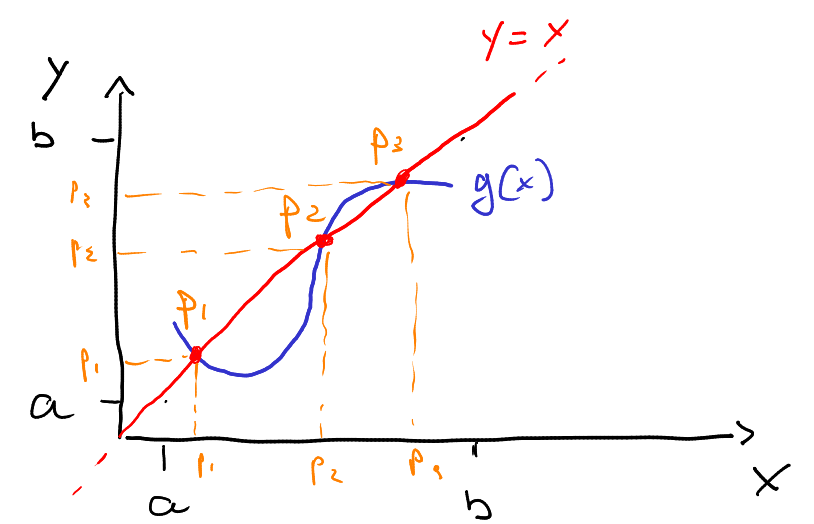
\includegraphics[width=0.5\textwidth]{img/2024-09-28-17-27-59.png}
\end{center}
Prendendo due dei punti fissi, $ p_1, p_2 $, notiamo che $ \frac{|g(p_1) - g(p_2)|}{|p_1 - p_2|} = \frac{|p_1 - p_2|}{|p_1 - p_2|} = 1 $, ma dato che la costante $ C $ deve essere minore di $ 1 $, abbiamo dimostrato l'assurdo. 
}
Manca la dimostrazione della garanzia dell'esistenza del punto fisso, che vedremo piu' avanti. (\ref{dimConvergPtFisso})

\subsubsection{Come controllare se una funzione differenziabile e' una mappa contrattiva}
Nella dimostrazione precedente e' apparsa una forma che somigliava molto a una derivata. Infatti, se la funzione $ g $ e' derivabile possiamo usare il seguente teorema:
\thm{}{
  Se una funzione $ g: [a,b] \to [a,b] $ e' differenziabile e esiste una costante $ C < 1 $ tale che $ \forall x \in [a,b]. |g'(x)|<C $, allora $ g $ e' una \textbf{mappa contrattiva}
}
\pf{Dimostrazione}{
  Per il teorema di Lagrange, $ \forall x < y \in [a,b]. \exists c \in [x,y]. g(y)-g(x) = g'(c)(y-x) $. Quindi, aggiungendo valori assoluti, $|g(y)-g(x)| = |g'(c)|\cdot |y-x| \leq C \cdot |y-x|$ per ipotesi. Quindi, per definizione, $ g $ e' una mappa contrattiva.
}

\subsection{Velocita' del miglioramento dell'approssimazione}
Chiamiamo l'errore assoluto $ |E_k| $ la differenza assoluta fra $ x_k $ e il valore effettivo del punto fisso $ p $.
\mprop{}{
  $ |E_{k+1}| \leq C|E_k| $, quindi 
  \[
  |E_k| \leq C^k|E_0|
  \]
  Dove $ E_0 = x_0 - p $.
}
Quindi per ogni iterazione, l'errore iniziale diminuisce almeno di un fattore $ C $ (che ricordo e' sempre $ <1 $ quindi e' una cosa buona). Cio' implica che piu' e' piccolo $ C $, piu' ci avviciniamo in fretta a $ p $. 
\pf{Dimostrazione}{
  Per definizione di errore $ E_{k+1} = x_{k+1} - p $, che possiamo riscrivere come $ g(x_k) - g(p) $, quindi per definizione di mappa contrattiva $ |E_{k+1}| = |g(x_k) - g(p)| \leq C|x_k - p| = C|E_k| $. Se sostituiamo $ k = 0 $ abbiamo il caso base:
  \[
  |E_1| \leq C|x_0 - p|
  \]
  Da cui ricorsivamente: 
  \[
    |E_k| \leq C|E_{k-1}| \leq C \cdot C|E_{k-2}| \leq ... \leq C \cdot ... \cdot C|E_0| = C^k|x_0 - p|
  \]
}

Ora siamo in grado di finire la dimostrazione di prima:
\pf{Diostrazione (convergenza)}{ \label{dimConvergPtFisso}
  Dato che $ C<1 $, se $ k \to +\infty $ allora $ C^k \to 0 $, quindi $ \lim_{k \to +\infty} |E_k| = \lim_{k \to +\infty} C^k|x_0 - p| = 0 $. Allora:
  \[
    x_k \xlongrightarrow{k \to +\infty} p
  \]
}

\section{Metodo di Newton}
Vediamo ora il metodo di Newton, che rispetto alla bisezione e' generalmente piu' veloce (ma non abbiamo la garanzia). Puo' essere dimostrato ricorrendo alle mappe contrattive o come approssimazione a linee tangenti, vediamo la prima:\\\\
Prendiamo una funzione differenziabile $ f $ e costruiamole una mappa contrattiva $ g $. Per migliorare l'efficenza, vogliamo fare in modo che la costante $ C $ abbia valore minimo dato un intorno della radice $ r $ di $ f $, come facciamo? Dato che $ C $ assume il valore della derivata massima della mappa, vogliamo fare in modo che la derivata di $ g $ sia minima per quell'intorno. Un modo per fare cio' e' assicurarci che $ g'(r) = 0 $, vediamo come:
\[
  g'(r) = 1 - w'(r)f(r) - w(r)f'(r) = 1 - w(r)f'(r)
\]
dato che $ f(r) = 0 $ per definizione, quindi:
\[
  w(r) = \frac{1}{f'(r)}
\]
Dato che non sappiamo il valore di $ r $, poniamo $ w(x) = \frac{1}{f'(x)} $ per ogni $ x $ nel dominio. Da notare che $ w(x) $ non esiste quando $ f'(x) = 0 $. Facendo cosi', la formula di iterazione diventa:
\[
  x_{k+1} = x_k - \frac{f(x_k)}{f'(x_k)}
\]
che e' la formula per il metodo di Newton.

